\documentclass[10pt,a4paper]{article}
\usepackage[margin=2cm]{geometry}
\usepackage{graphicx,booktabs,amsmath,float,array}
\usepackage[hidelinks]{hyperref}
\title{VLSI Design Course Project\\Part I: 4-bit Carry Look-Ahead Adder}
\author{Bhargav, Roll No. 2025102061\\IIIT Hyderabad, Monsoon 2026}
\date{}
\begin{document}
\maketitle
\tableofcontents

\section*{Summary of results}
All values below are from ngspice runs, and post-layout values use netlists extracted by MAGIC. Unless stated otherwise, delays are worst-case over all 4608 single-input transitions, measured from the 50\% point at the adder input pin to the final 50\% crossing at the output. Inputs are driven by a finite inverter, and each output drives the $W_p/W_n=20\lambda/10\lambda$ inverter.

\begin{table}[H]\centering
\small
\caption{Final design}
\begin{tabular}{p{7.2cm}p{8.2cm}}
\toprule
\textbf{Quantity} & \textbf{Value} \\
\midrule
Architecture & Static CMOS prefix CLA with dual-rail AOI22 sum; TSPC flip-flops \\
Adder transistors / registered transistors & 194 / 348 \\
Schematic worst-case delay & 516.3 ps \\
Post-layout worst single-input transition & 579.88 ps (a1 rise to s3 rise, A=0001 B=0101 C0=0) \\
Post-layout worst found overall, tpd,max & 589.85 ps (several inputs changing; from a sample) \\
Course hint vector, post-layout worst & 454.1 ps \\
Flip-flop post-layout tcq / tsetup / thold & 204.2 / 38.0 / 45.7 ps \\
fmax by course formula & 1.4847 GHz (T = 673.6 ps) \\
Verified limit, extracted registered circuit & 1.1467 GHz (T = 872.1 ps) \\
Pavg at verified limit, random and critical vectors & 3.3899 mW \\
PDP (Pavg x tpd,max) & 1999.51 fJ \\
Layout area, adder / registered & 2937 / 7006 um2 \\
ADP, adder & 1732 um2 ns \\
DRC errors, adder and registered & 0 and 0 \\
\bottomrule
\end{tabular}
\end{table}

\noindent\textbf{Points to note.} (1) The course formula gives a higher frequency than the circuit achieves: At the course-formula period (673.6 ps) the extracted registered circuit gave 264 wrong output samples, so that frequency is \emph{not} reliable for this design. The formula leaves out clock-to-Q delay. (2) The hint vector is not the worst case. The slowest arcs start at operand bits, not at $C_0$. (3) MAGIC has no usable resistance extraction here, so resistance is bounded by simulation in Section~\ref{sec:res}, not extracted. (4) Figure 1(i) shows no register on $C_{in}$; a ninth input flip-flop was added. (5) The load sentence names sum bits only; $C_4$ also drives the inverter here.

\section{Literature review}
Twenty provided papers were read. Few state the output load, input driver or the transitions tested, so their delay figures are not comparable with this work or with each other.
\begin{itemize}
\item \textbf{OR-type propagate:} Miao and Li~\cite{miao} replace XOR with NOR in the carry path and name a path from B0 through C3 to S3 as the longest. Both ideas were tested here, and the worst paths here also start at operand bits.
\item \textbf{Mirror and flat carry gates:} Hasan et al.~\cite{hasan} build $C_4$ as one nested gate. Measured stacks here show why this is costly: a worst-position NOR5 is 4.6 FO4 at 180 nm.
\item \textbf{Reduced-swing styles:} GDI and pass-transistor papers (Dipto 2020, Hossain 2020, Joy 2023, Chezhiyan 2025) report gains against their own baselines at 90 nm. One of these (Chezhiyan and Bommi 2025) itself lists static CMOS as fastest. They were not adopted.
\item \textbf{Dynamic logic:} Zlatanovici et al.~\cite{zlat} show dynamic logic winning at 64 bits, and static preferred at long cycle times. Efstathiou et al.~\cite{efst} report only 4.73\% gain at 8 bits from a Ling-style split. Neither applies directly at 4 bits.
\item \textbf{False sums:} Nyathi and Mutumba~\cite{nyathi} show sums switching before carries settle, which is why delay here is measured at the final crossing.
\item \textbf{Single-threshold limit:} MT-CMOS and dual-mode designs (Sivakumar 2013, Chaitanya Kumar 2014) need low-threshold devices that the provided model does not offer.
\end{itemize}
Full notes, with source pages, are in \texttt{explanation/research/literature\_review.md}.

\section{Proposed structure}
\subsection{Equations and structure}
With $p_i=a_i\oplus b_i$, $g_i=a_ib_i$, $t_i=a_i+b_i$, the carries can use $t_i$ in place of $p_i$, because the two differ only when $g_i=1$. XOR is then needed only for the sum, $S_i=p_i\oplus c_i$, so the carry path is free of a slow XOR. This idea follows Miao and Li~\cite{miao}.

The carries are computed as a prefix tree with $C_0$ entering last:
\[G_{1:0}=g_1+t_1g_0,\quad T_{1:0}=t_1t_0,\quad G_{3:2}=g_3+t_3g_2,\quad T_{3:2}=t_3t_2,\]
\[G_{3:0}=G_{3:2}+T_{3:2}G_{1:0},\quad G_{2:0}=g_2+t_2G_{1:0},\quad C_{k}=G_{k-1:0}+T_{k-1:0}C_0.\]
Each level is inverting, so polarity alternates: NAND2 and NOR2 give active-low $\bar g,\bar t$; OAI21 and NOR2 give active-high level 1; AOI21 and NAND2 give active-low level 2; a final OAI21 with $\bar C_0$ gives each carry. $C_0$ passes through one inverter and one gate.

\begin{figure}[H]\centering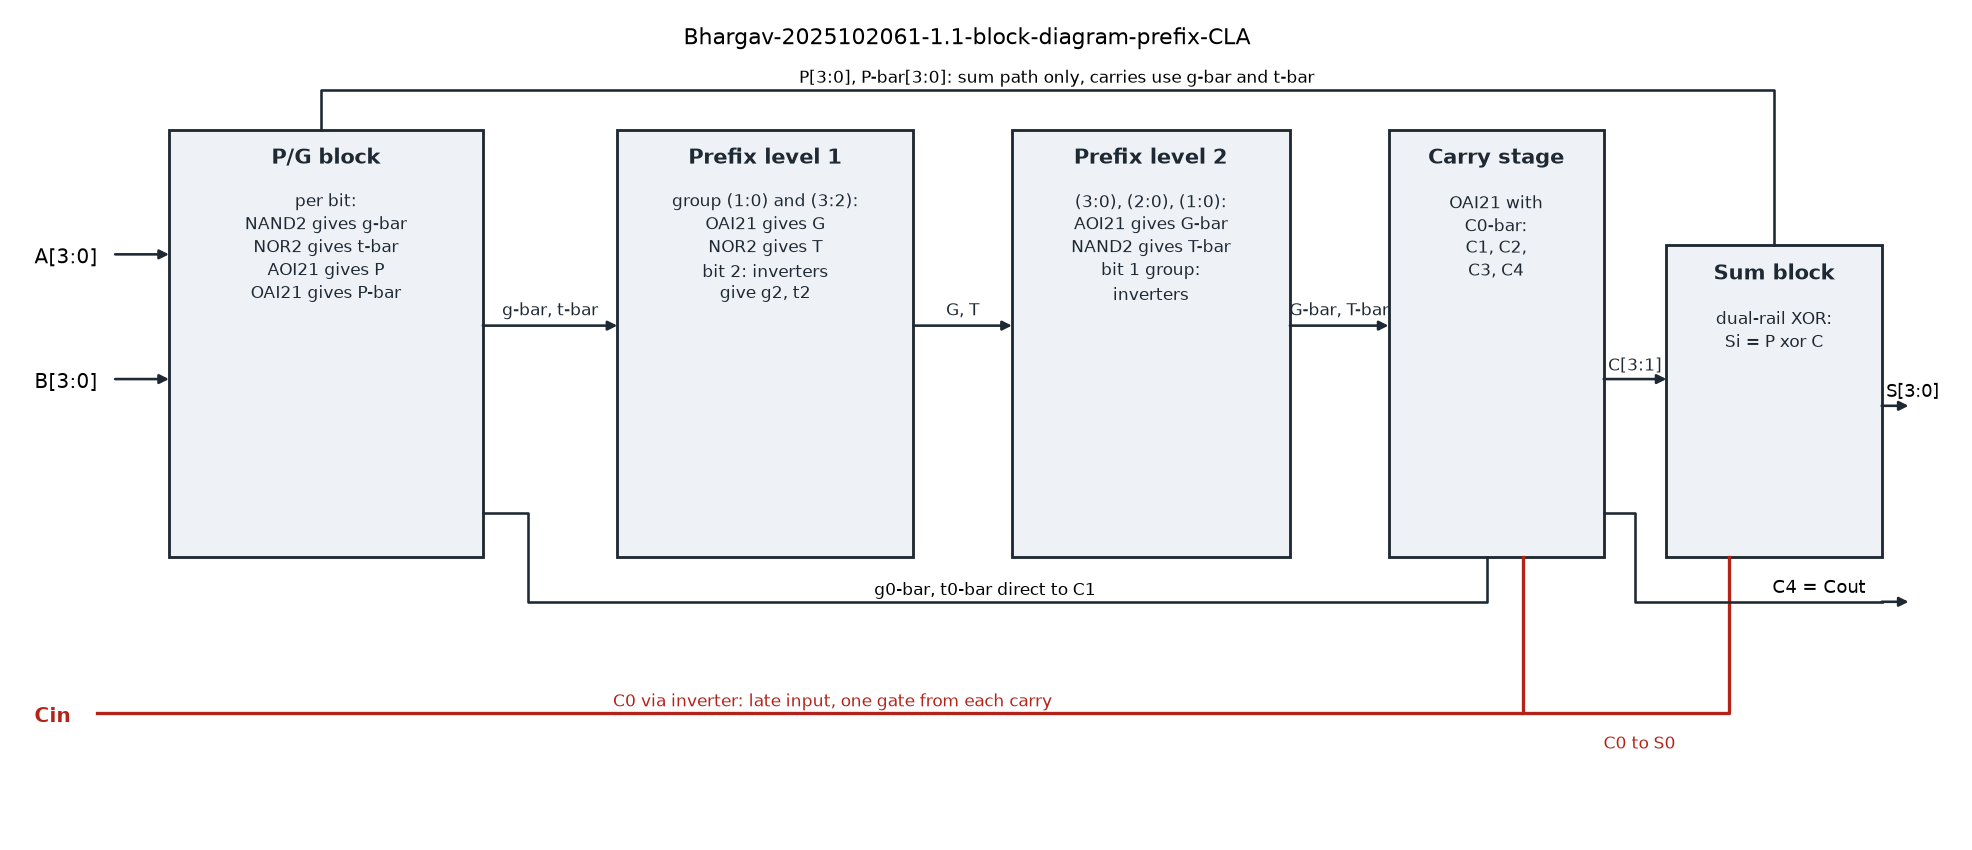
\includegraphics[width=\textwidth]{figures/block_diagram.png}\caption{Block-level architecture. Signals are named as in the netlists.}\end{figure}

\subsection{How this architecture was chosen}
Six architectures were simulated at unit sizing, over all 4608 single-input transitions. Delay from the driver input also charges each design for its input capacitance.

\begin{table}[H]\centering
\footnotesize
\caption{Unit-size comparison, schematic, all single-input transitions}
\begin{tabular}{lrrrrr}
\toprule
\textbf{Candidate} & \textbf{T} & \textbf{Width (lambda)} & \textbf{Worst pin (ps)} & \textbf{From driver (ps)} & \textbf{Hint vector (ps)} \\
\midrule
C1 & 208 & 5260 & 771.3 & 832.5 & 421.4 \\
C2 & 170 & 5470 & 764.0 & 840.6 & 577.2 \\
R & 172 & 5160 & 727.0 & 803.5 & 574.2 \\
C3 & 170 & 4800 & 796.4 & 873.1 & 623.5 \\
C4 & 194 & 4930 & 658.9 & 735.5 & 360.0 \\
E & 144 & 3480 & 799.8 & 882.2 & 629.1 \\
R/tg & 164 & 4560 & 698.8 & 787.0 & 542.1 \\
R/static12 & 180 & 5280 & 726.8 & 803.4 & 574.2 \\
R/nand4 & 196 & 5360 & 740.4 & 848.8 & 605.5 \\
\bottomrule
\end{tabular}
\end{table}

C1 is the textbook XOR and NAND-NAND design; C2 uses one complex gate per carry, up to a 5-high stack; R is C2 with $C_4$ from a mirror gate over $C_2$; C3 limits stacks to 3; C4 is the prefix tree; E is a static Manchester chain. A first-order logical-effort estimate had placed flat designs ahead of the prefix tree. Measurement contradicted it, so the estimate was dropped. C4 was the fastest and was carried forward. Two sum cells, a dual-rail AOI22 XOR and a transmission-gate XOR, were within 3 ps of each other after sizing on schematic. The AOI22 version was faster after layout, and speed is the primary objective, so it was kept. Only the chosen design is reported post-layout.

\section{Design details: topology and sizing}
\subsection{Adder}
Sizes come from a search minimising worst-case delay from the driver input, confirmed against every input-output class, then repeated with wire capacitance extracted from the layout. Widths below are in $\lambda$ ($\lambda=0.09\,\mu$m); every channel length is $2\lambda$, equal for NMOS and PMOS. Multiple widths are the different series positions in a stack.

\begin{table}[H]\centering
\scriptsize
\caption{Final adder sizing, every instance}
\begin{tabular}{llcrll}
\toprule
\textbf{Instance} & \textbf{Cell} & \textbf{Output} & \textbf{T} & \textbf{NMOS W} & \textbf{PMOS W} \\
\midrule
nand0 & nand2 & g0b & 4 & 25 & 25 \\
nor0 & nor2 & t0b & 4 & 16 & 62 \\
aoi0 & aoi21 & p0 & 6 & 4/8 & 16 \\
oai0 & oai21 & p0b & 6 & 8 & 8/16 \\
nand1 & nand2 & g1b & 4 & 25 & 25 \\
nor1 & nor2 & t1b & 4 & 20 & 78 \\
aoi1 & aoi21 & p1 & 6 & 4/8 & 16 \\
oai1 & oai21 & p1b & 6 & 8 & 8/16 \\
nand2 & nand2 & g2b & 4 & 25 & 25 \\
nor2 & nor2 & t2b & 4 & 12 & 50 \\
aoi2 & aoi21 & p2 & 6 & 8/16 & 32 \\
oai2 & oai21 & p2b & 6 & 16 & 16/32 \\
nand3 & nand2 & g3b & 4 & 20 & 20 \\
nor3 & nor2 & t3b & 4 & 12 & 50 \\
aoi3 & aoi21 & p3 & 6 & 10/20 & 40 \\
oai3 & oai21 & p3b & 6 & 20 & 20/40 \\
invc0 & inv & c0b & 2 & 10 & 20 \\
g10 & oai21\_fn & g1\_0 & 6 & 25 & 25/50 \\
t10 & nor2 & t1\_0 & 4 & 16 & 62 \\
g32 & oai21 & g3\_2 & 6 & 16 & 16/32 \\
t32 & nor2 & t3\_2 & 4 & 8 & 32 \\
ig2 & inv & g2 & 2 & 12 & 25 \\
it2 & inv & t2 & 2 & 20 & 39 \\
g30 & aoi21\_fnp & g3\_0b & 6 & 4/8 & 16 \\
t30 & nand2 & t3\_0b & 4 & 8 & 8 \\
g20 & aoi21\_fnp & g2\_0b & 6 & 10/20 & 40 \\
t20 & nand2 & t2\_0b & 4 & 25 & 25 \\
ig10 & inv & g1\_0b & 2 & 10 & 20 \\
it10 & inv & t1\_0b & 2 & 16 & 31 \\
c1 & oai21 & c1 & 6 & 10 & 10/20 \\
c2 & oai21\_fn & c2 & 6 & 25 & 25/50 \\
c3 & oai21\_fn & c3 & 6 & 25 & 25/50 \\
c4g & oai21\_fnp & c4 & 6 & 16 & 16/32 \\
x0 & xor\_aoi22 & s0 & 10 & 5/25 & 10/50 \\
x1 & xor\_aoi22 & s1 & 10 & 6/20 & 13/40 \\
x2 & xor\_aoi22 & s2 & 10 & 12/16 & 25/32 \\
x3 & xor\_aoi22 & s3 & 10 & 10 & 20 \\
\bottomrule
\end{tabular}
\end{table}

\begin{figure}[H]\centering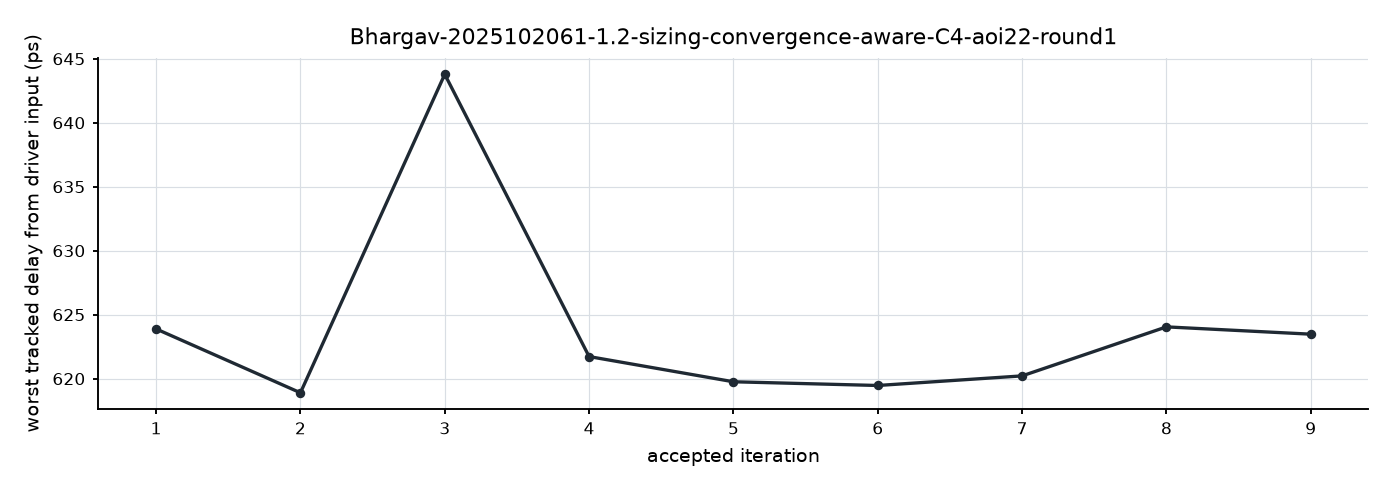
\includegraphics[width=0.82\textwidth]{figures/convergence.png}\caption{Layout-aware sizing, first round. Each point is an accepted step.}\end{figure}

\subsection{Transistor-level schematics}
Each drawing shows exactly the netlist's devices, terminals and sizes. All final cells are in \texttt{part1/schematics/transistor\_level/final/}. Representative cells follow.

\begin{figure}[H]\centering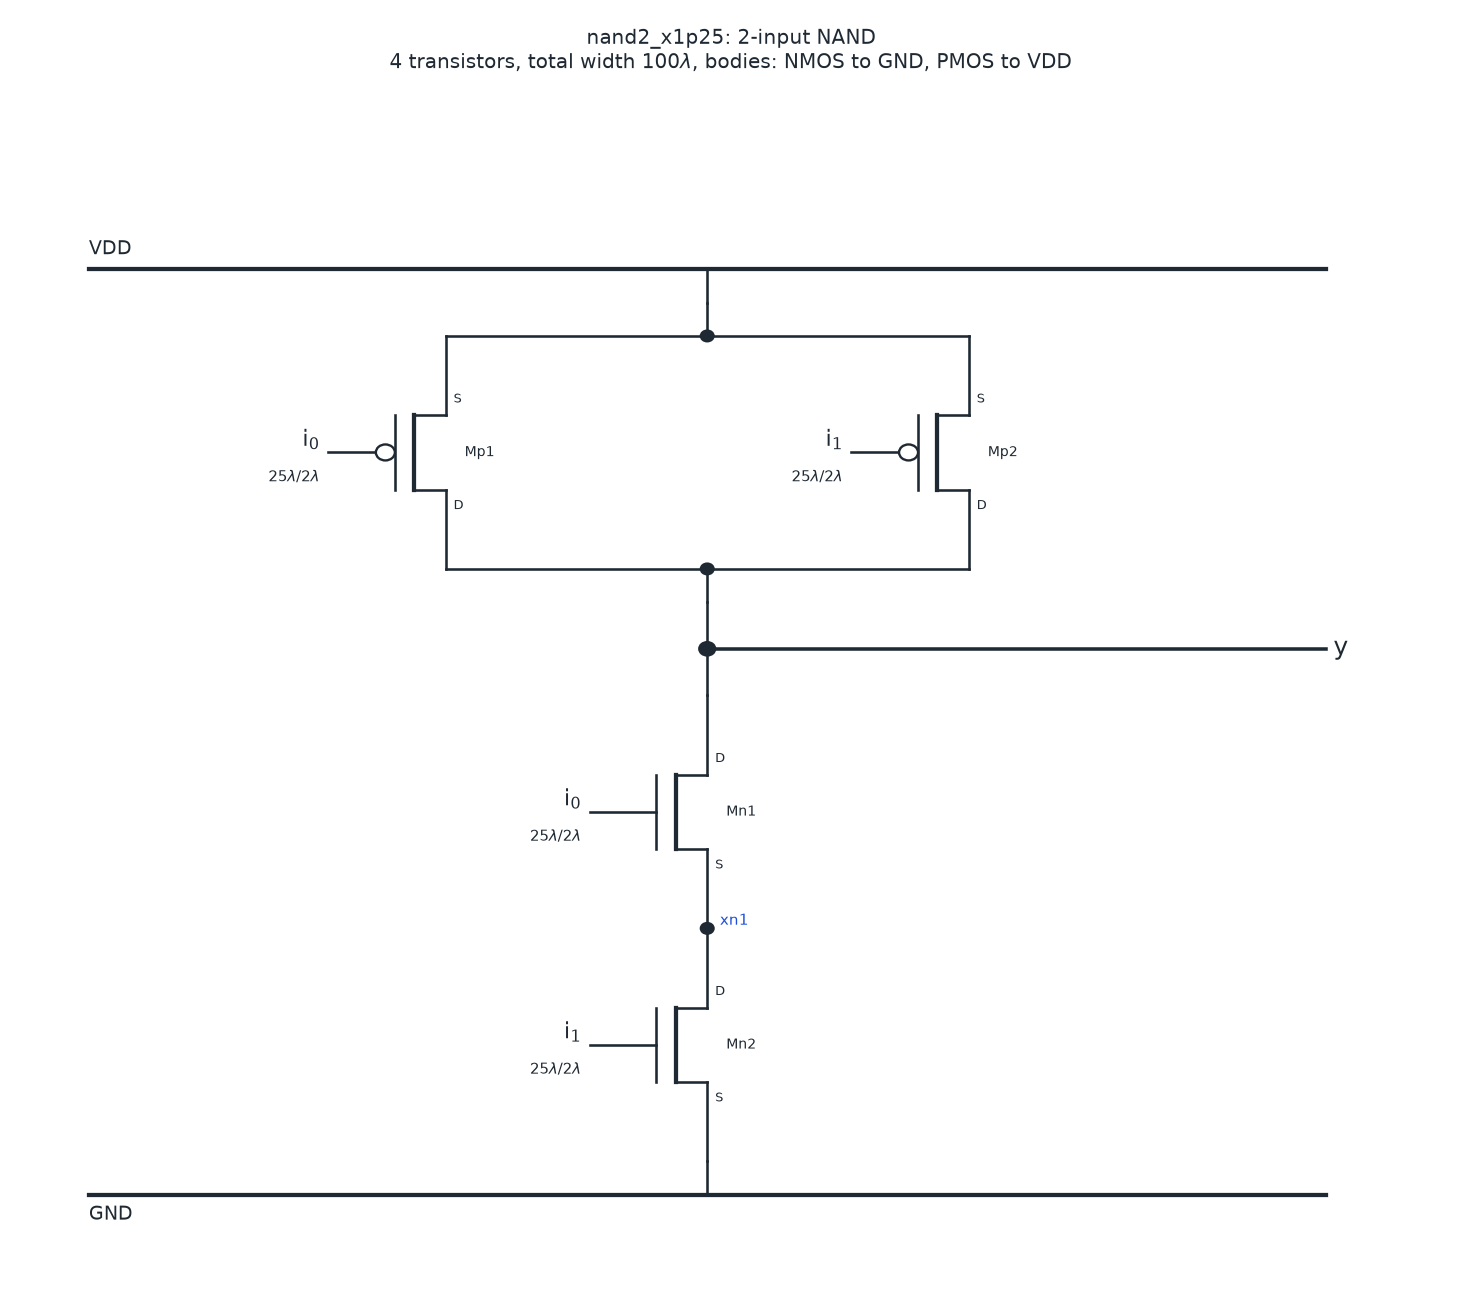
\includegraphics[width=0.48\textwidth]{figures/../../schematics/transistor_level/final/nand2_x1p25.png}\caption{NAND2 for generate, bit 0 (nand2\_x1p25).}\end{figure}
\begin{figure}[H]\centering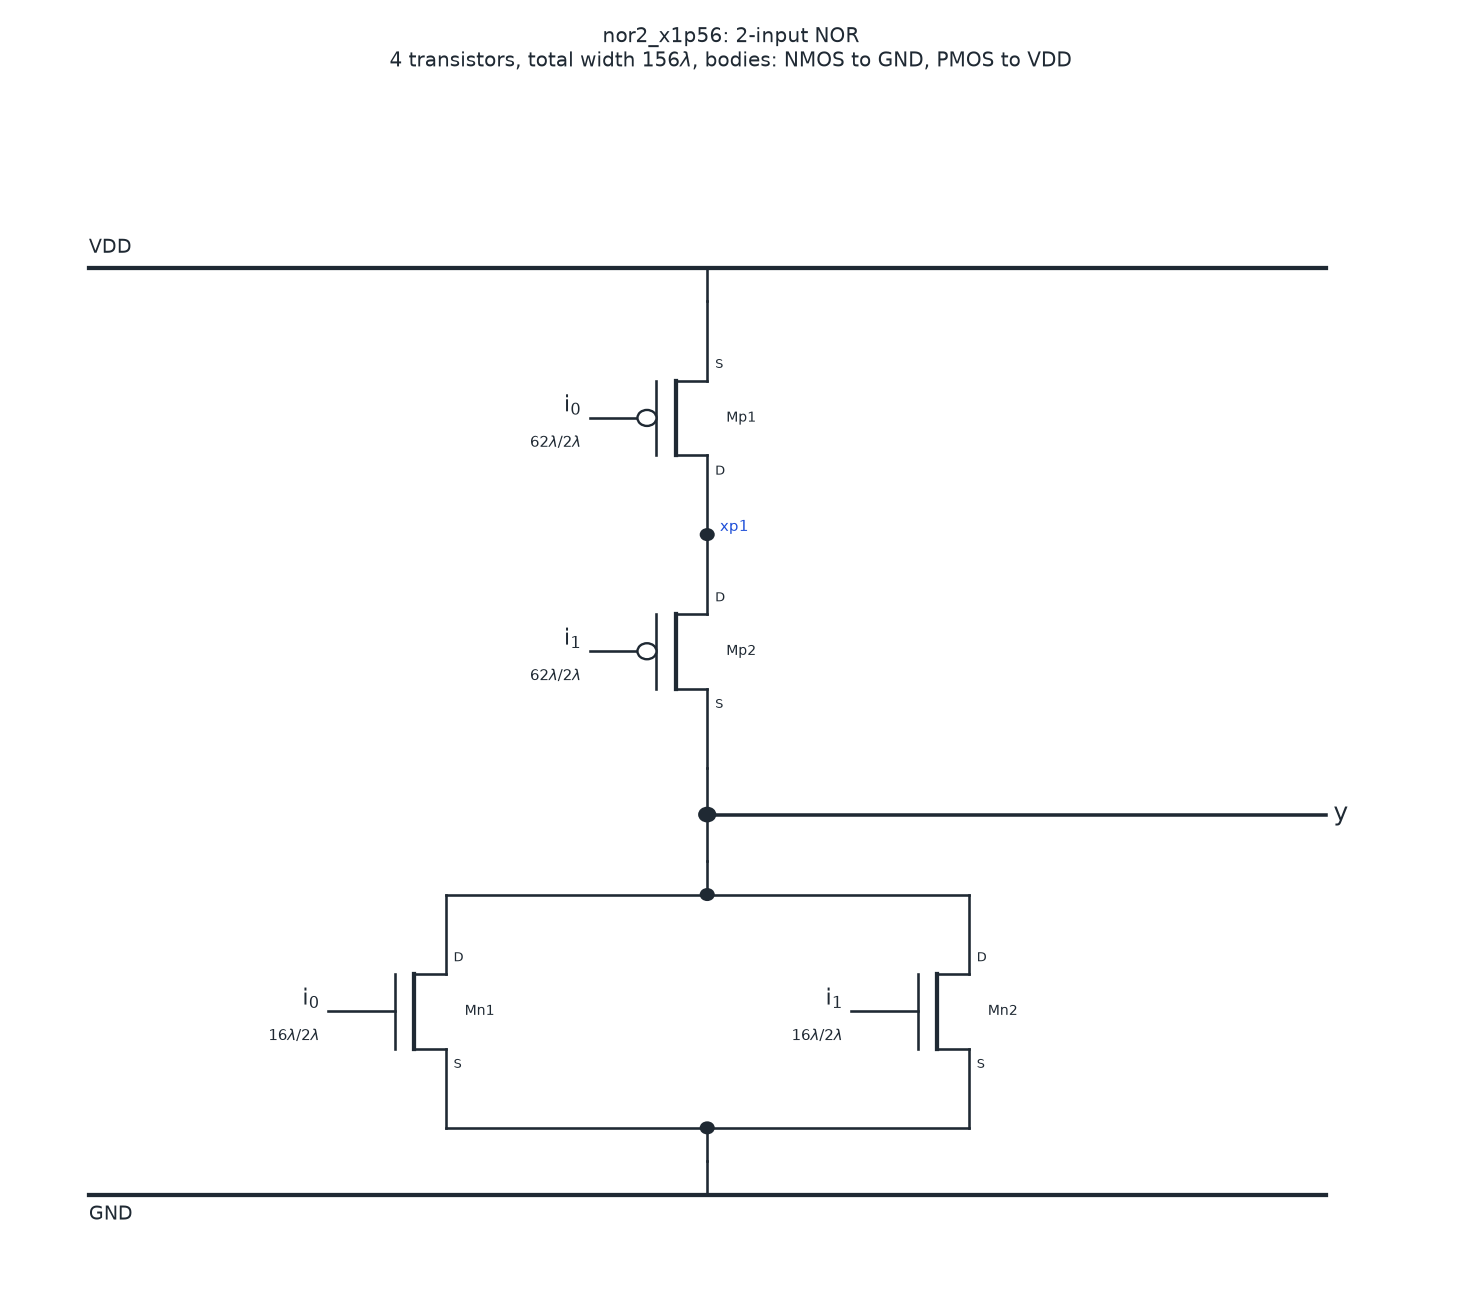
\includegraphics[width=0.48\textwidth]{figures/../../schematics/transistor_level/final/nor2_x1p56.png}\caption{NOR2 for OR-type propagate, bit 0 (nor2\_x1p56).}\end{figure}
\begin{figure}[H]\centering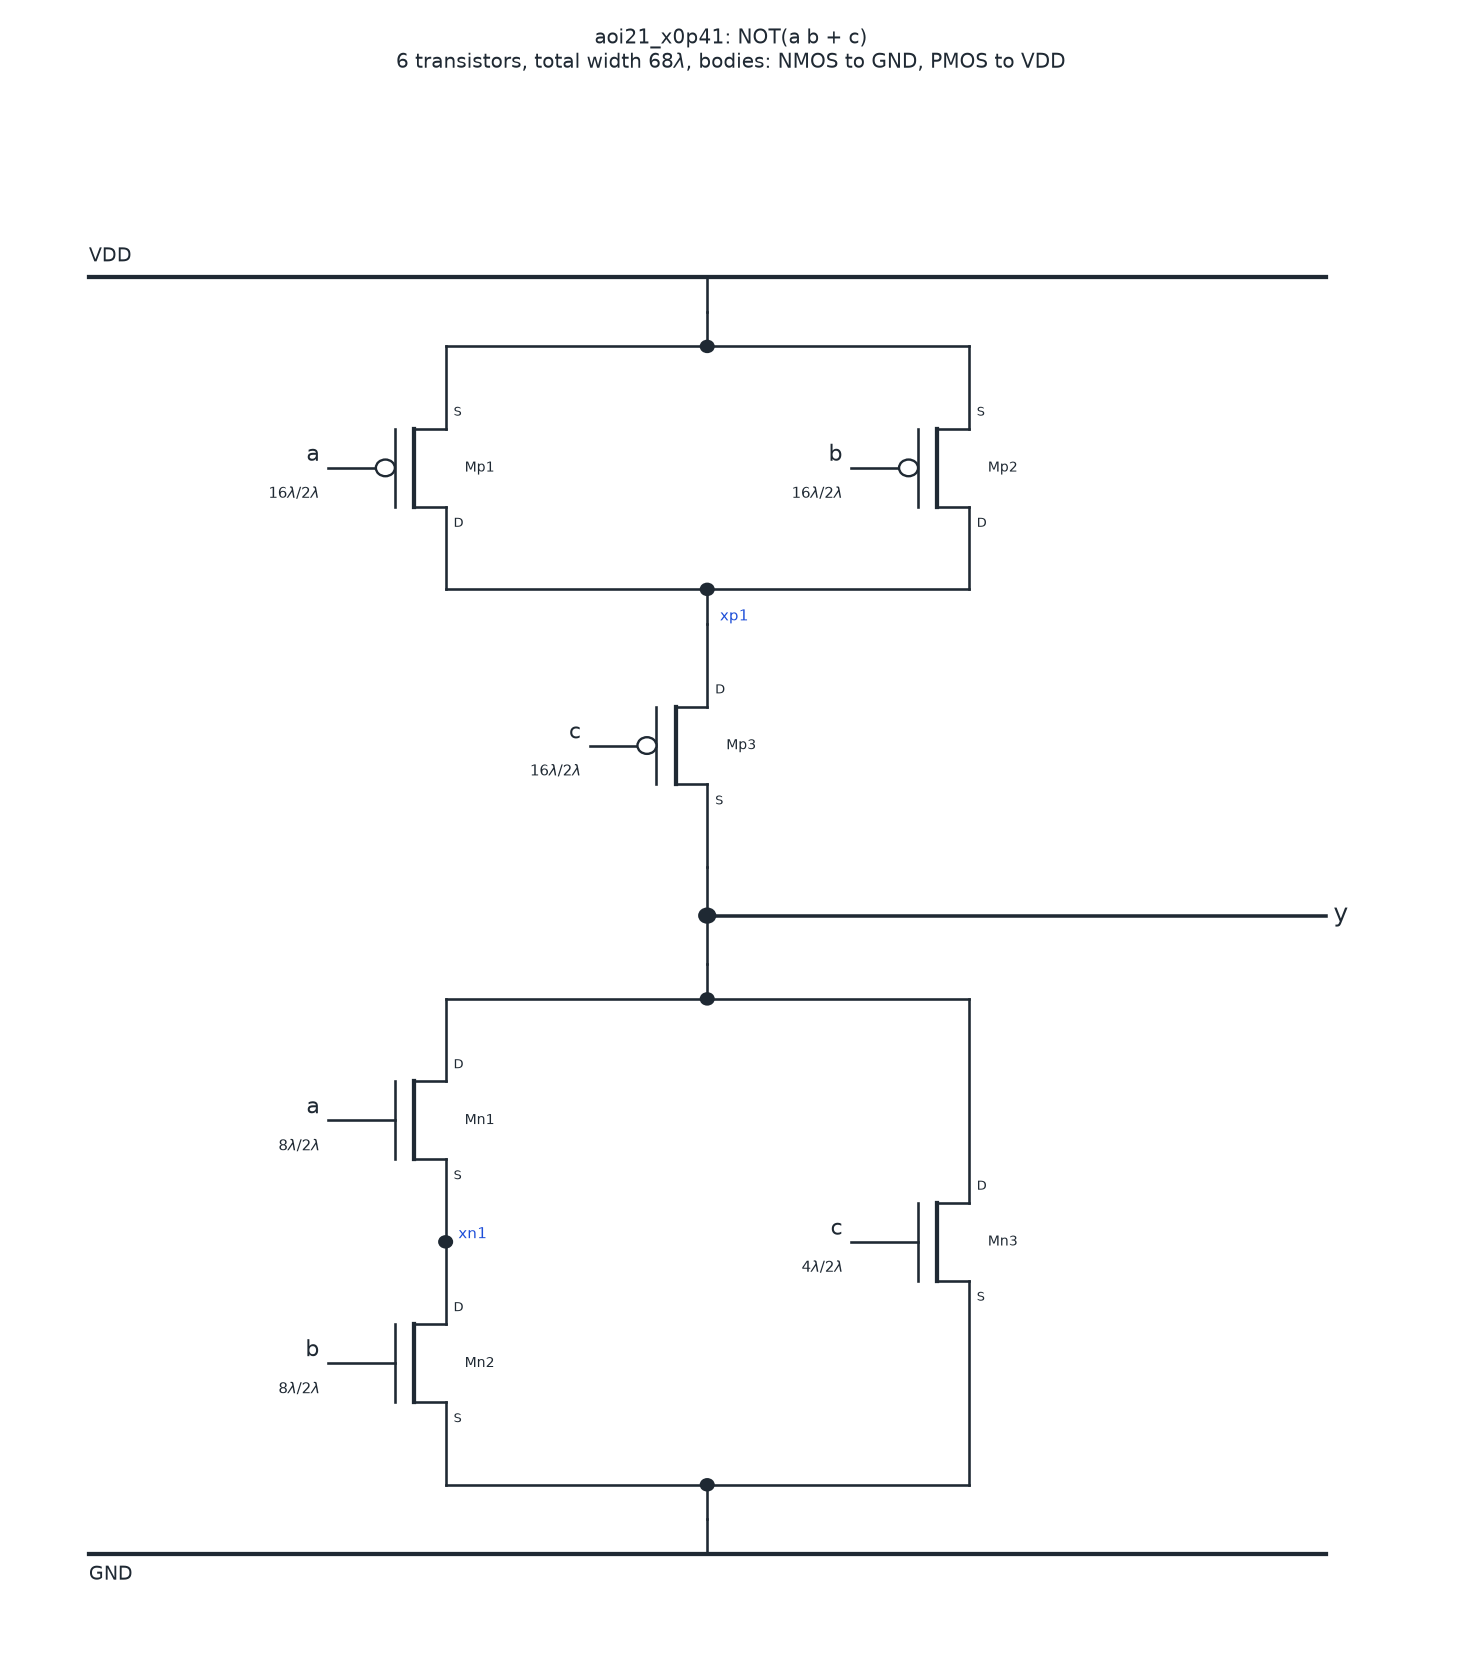
\includegraphics[width=0.48\textwidth]{figures/../../schematics/transistor_level/final/aoi21_x0p41.png}\caption{AOI21 for P, bit 0 (aoi21\_x0p41).}\end{figure}
\begin{figure}[H]\centering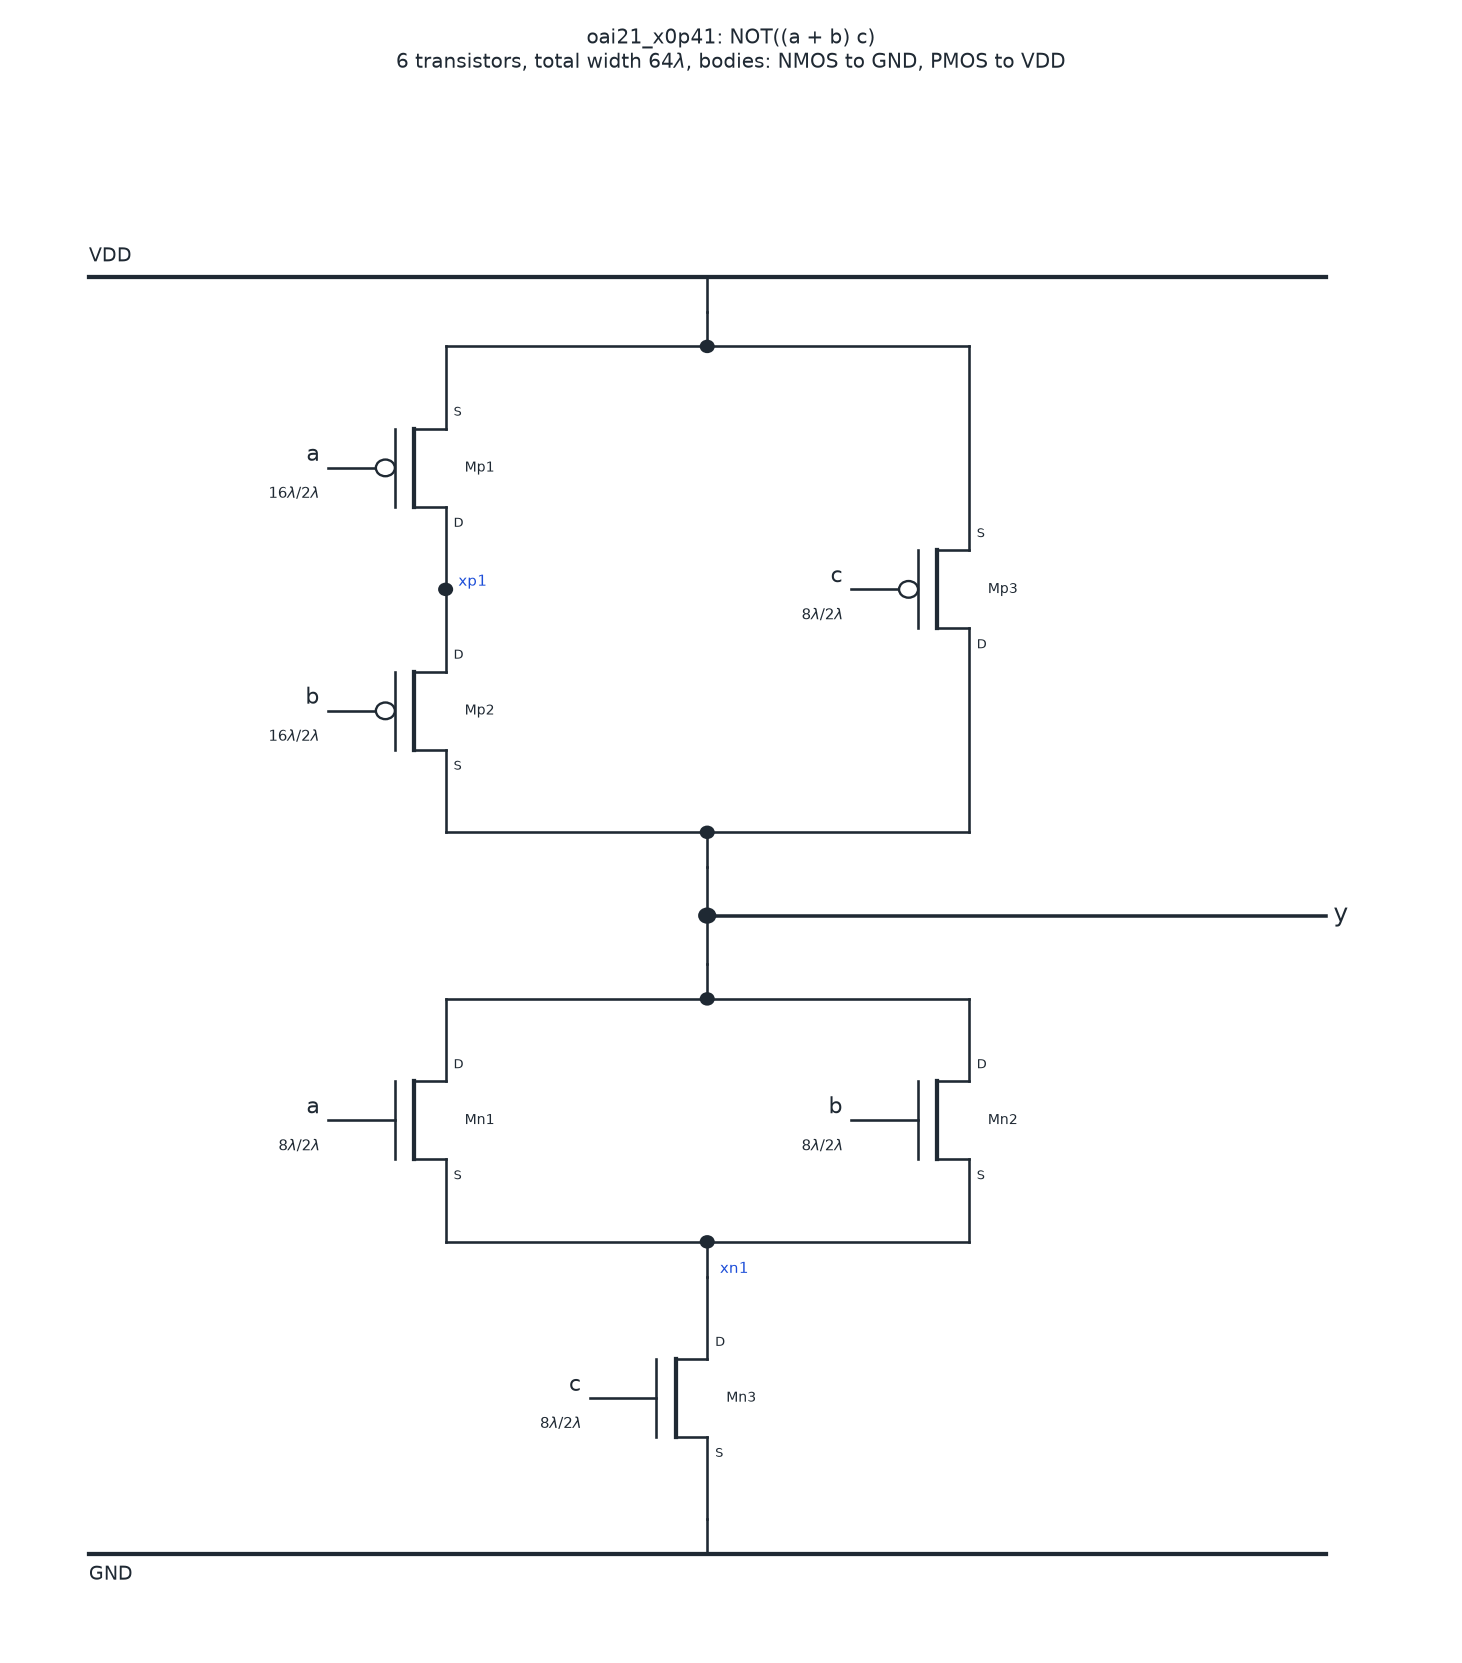
\includegraphics[width=0.48\textwidth]{figures/../../schematics/transistor_level/final/oai21_x0p41.png}\caption{OAI21 for P-bar, bit 0 (oai21\_x0p41).}\end{figure}
\begin{figure}[H]\centering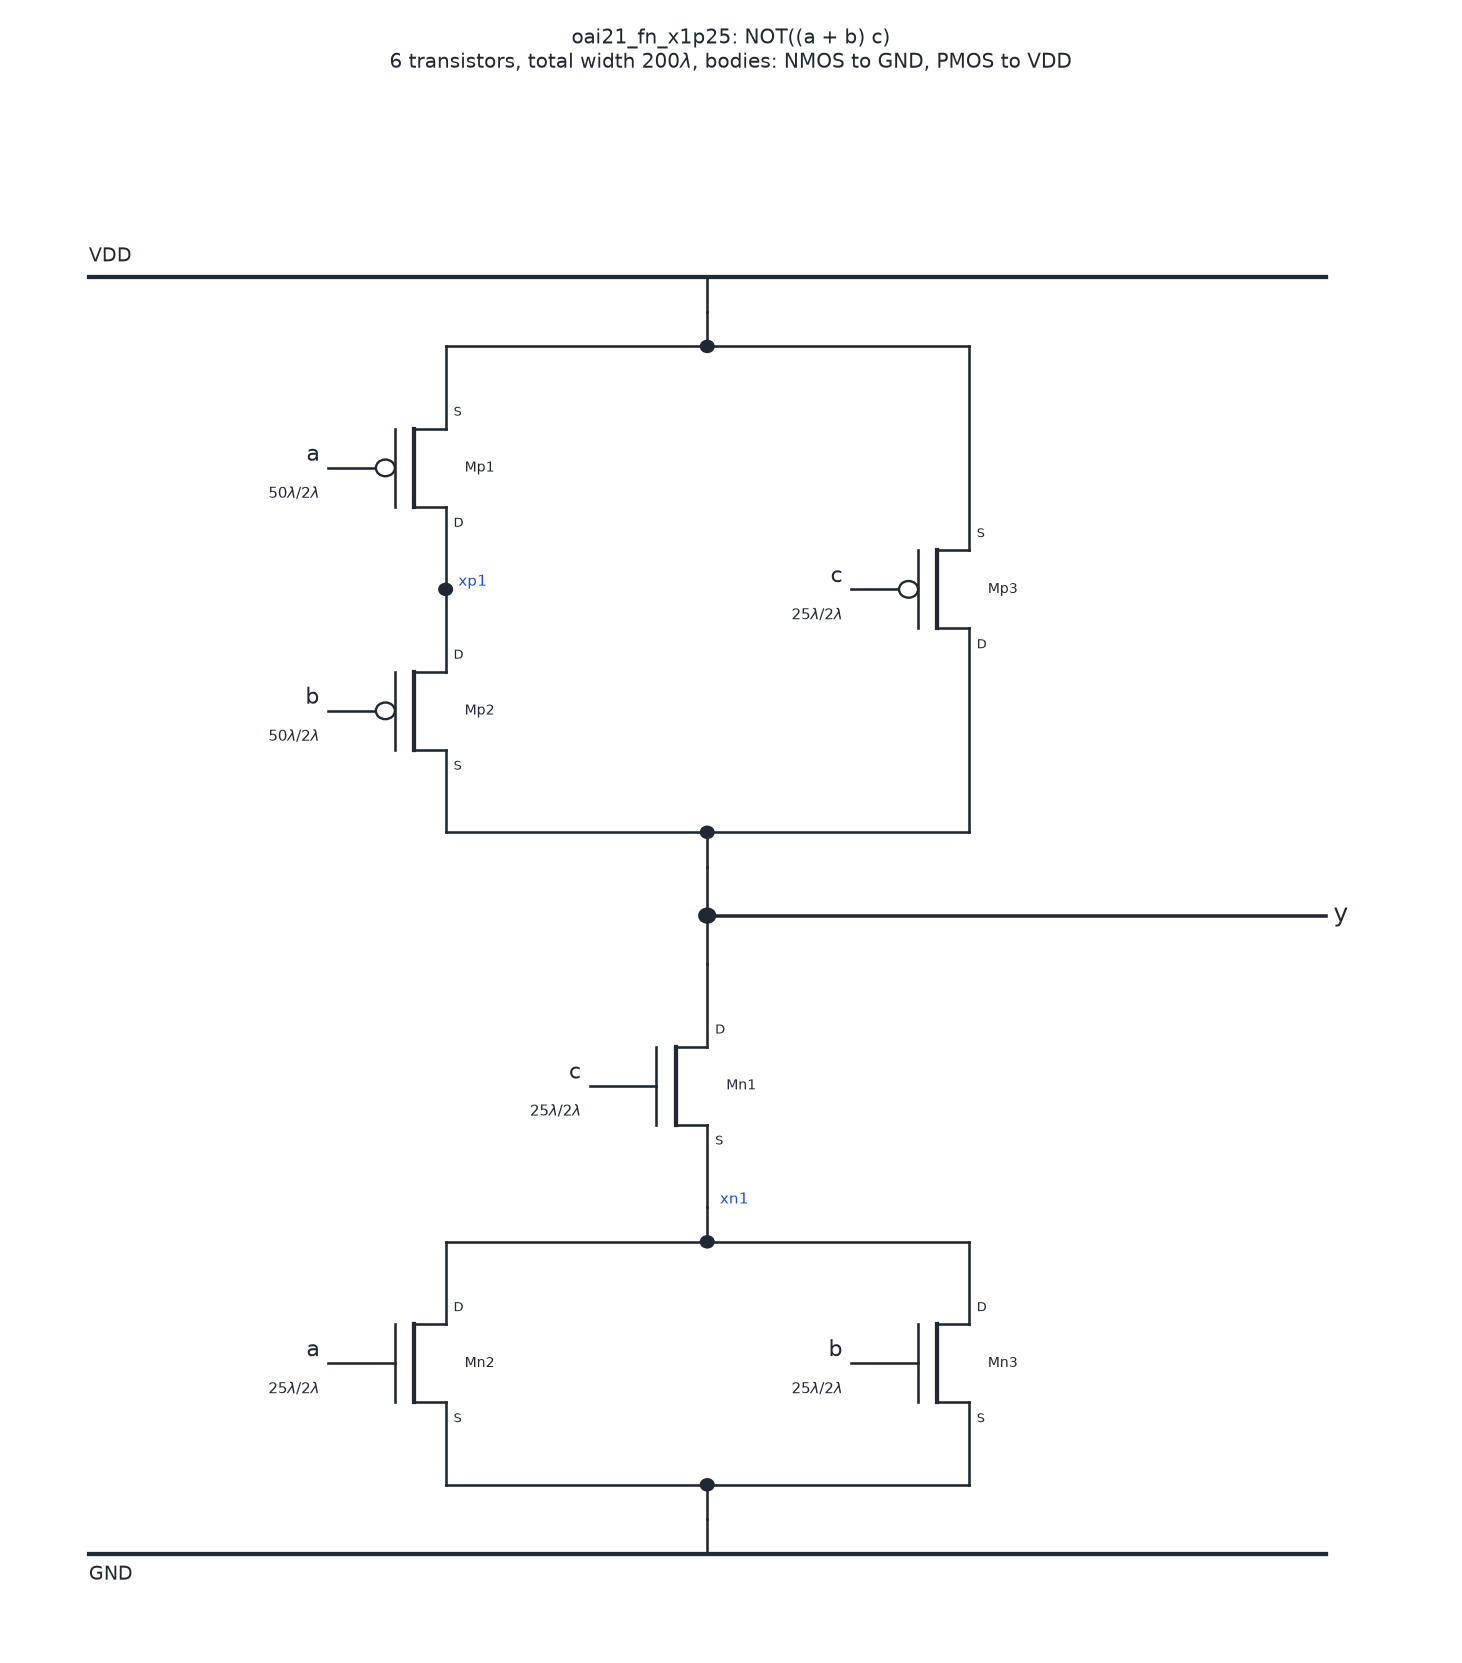
\includegraphics[width=0.48\textwidth]{figures/../../schematics/transistor_level/final/oai21_fn_x1p25.png}\caption{Prefix OAI21, G(1:0) (oai21\_fn\_x1p25).}\end{figure}
\begin{figure}[H]\centering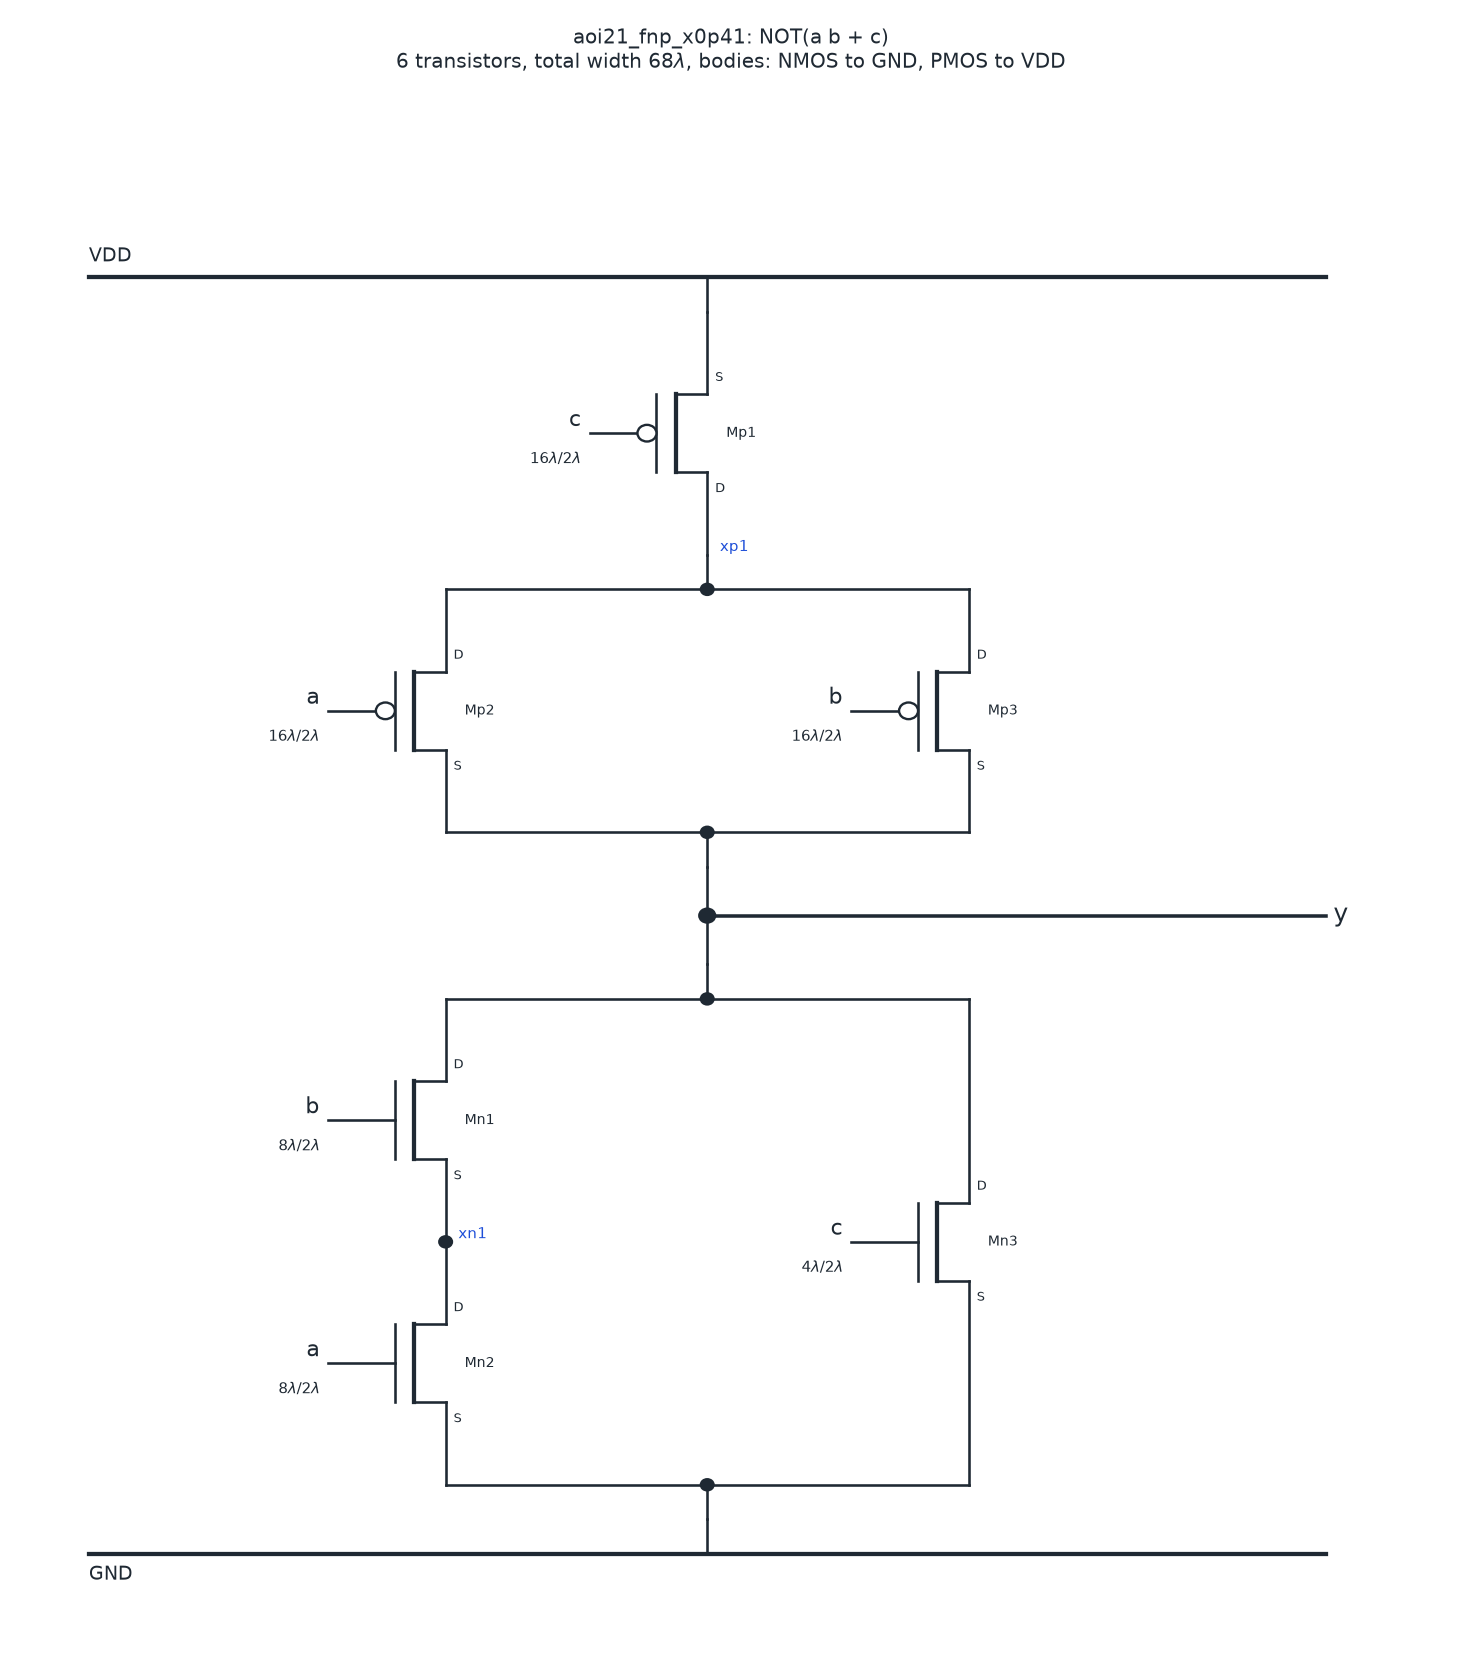
\includegraphics[width=0.48\textwidth]{figures/../../schematics/transistor_level/final/aoi21_fnp_x0p41.png}\caption{Prefix AOI21, G-bar(3:0) (aoi21\_fnp\_x0p41).}\end{figure}
\begin{figure}[H]\centering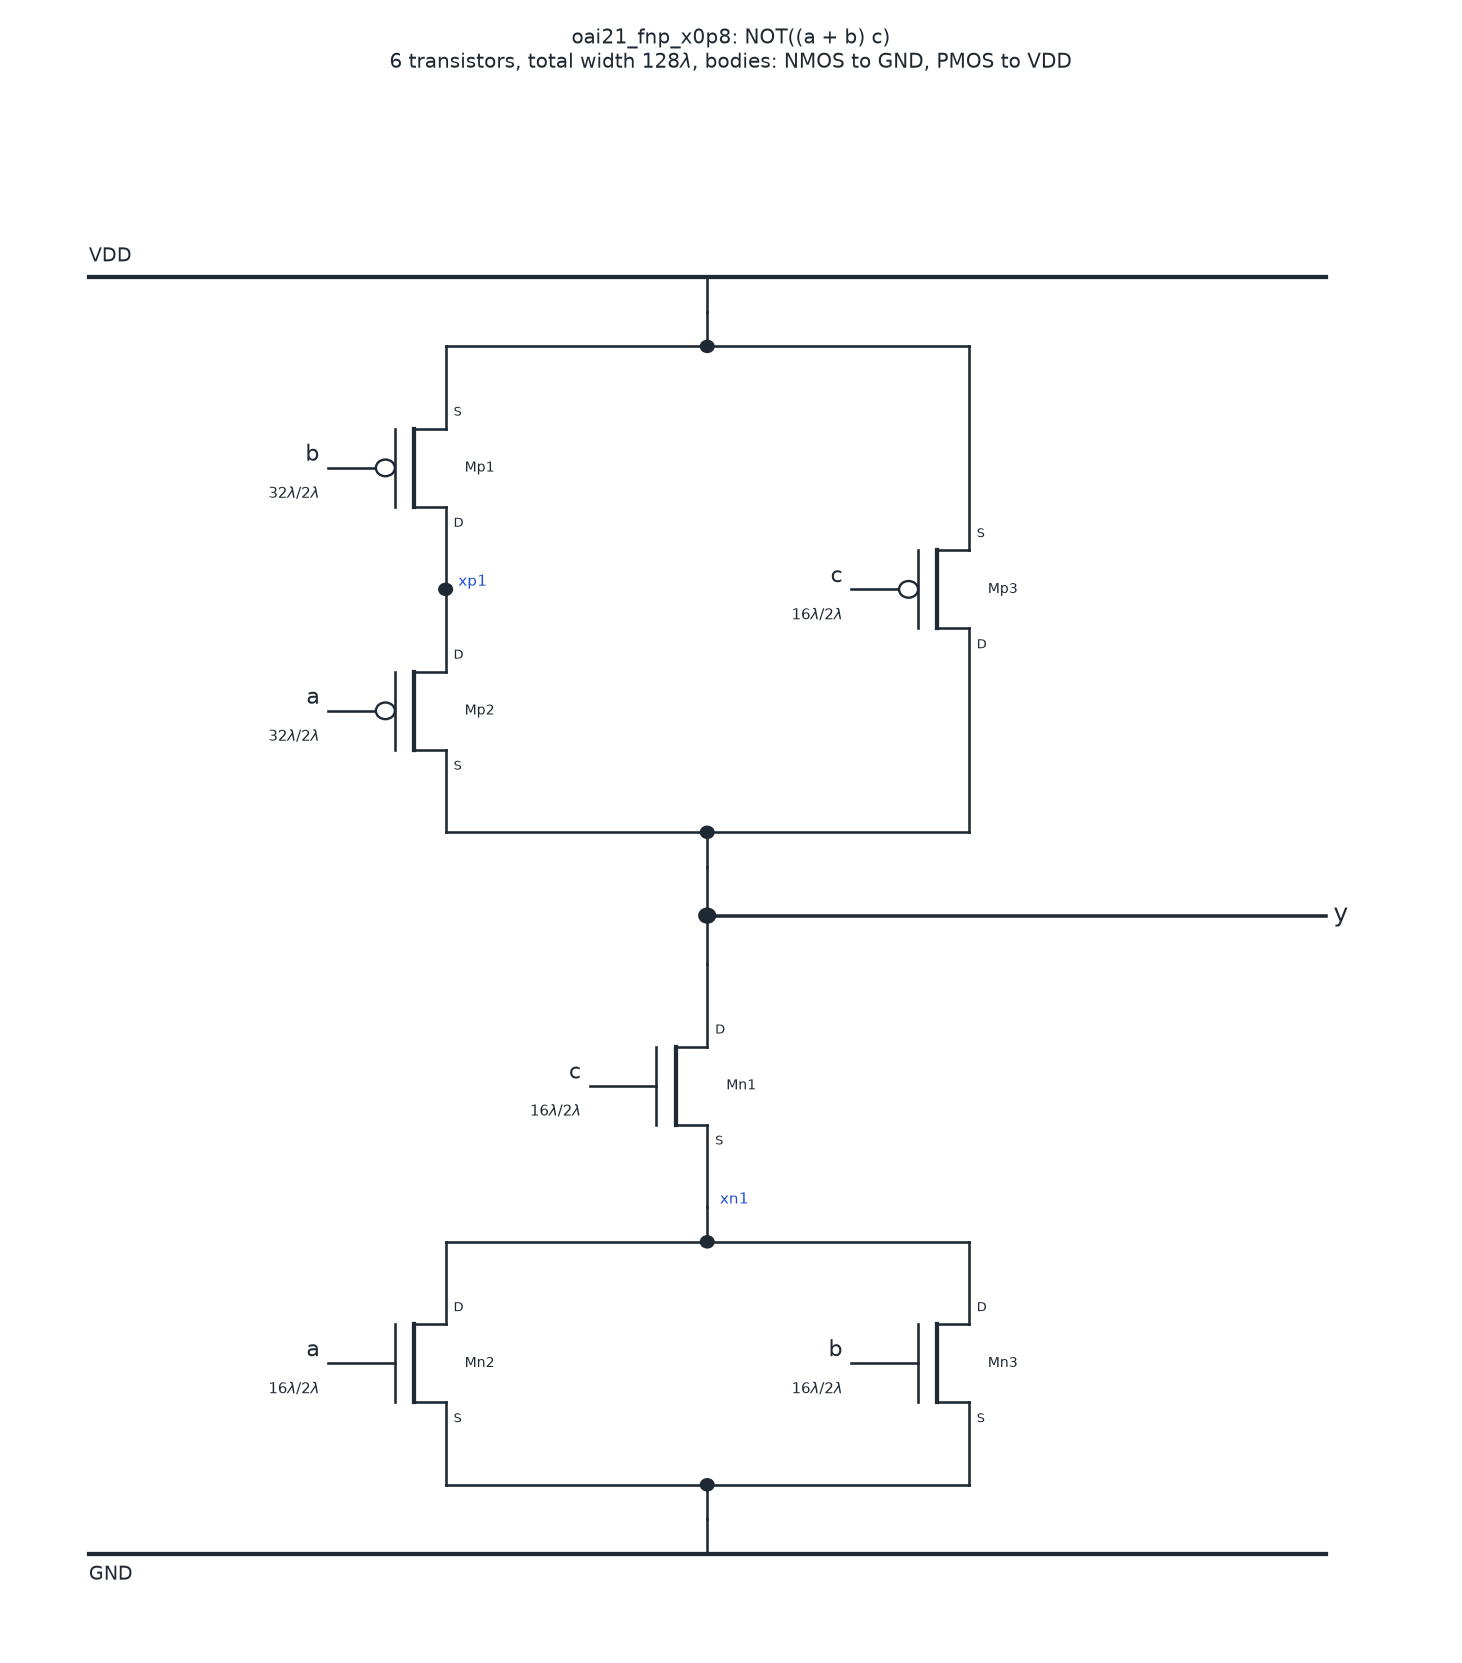
\includegraphics[width=0.48\textwidth]{figures/../../schematics/transistor_level/final/oai21_fnp_x0p8.png}\caption{Final carry OAI21, C4 (oai21\_fnp\_x0p8).}\end{figure}
\begin{figure}[H]\centering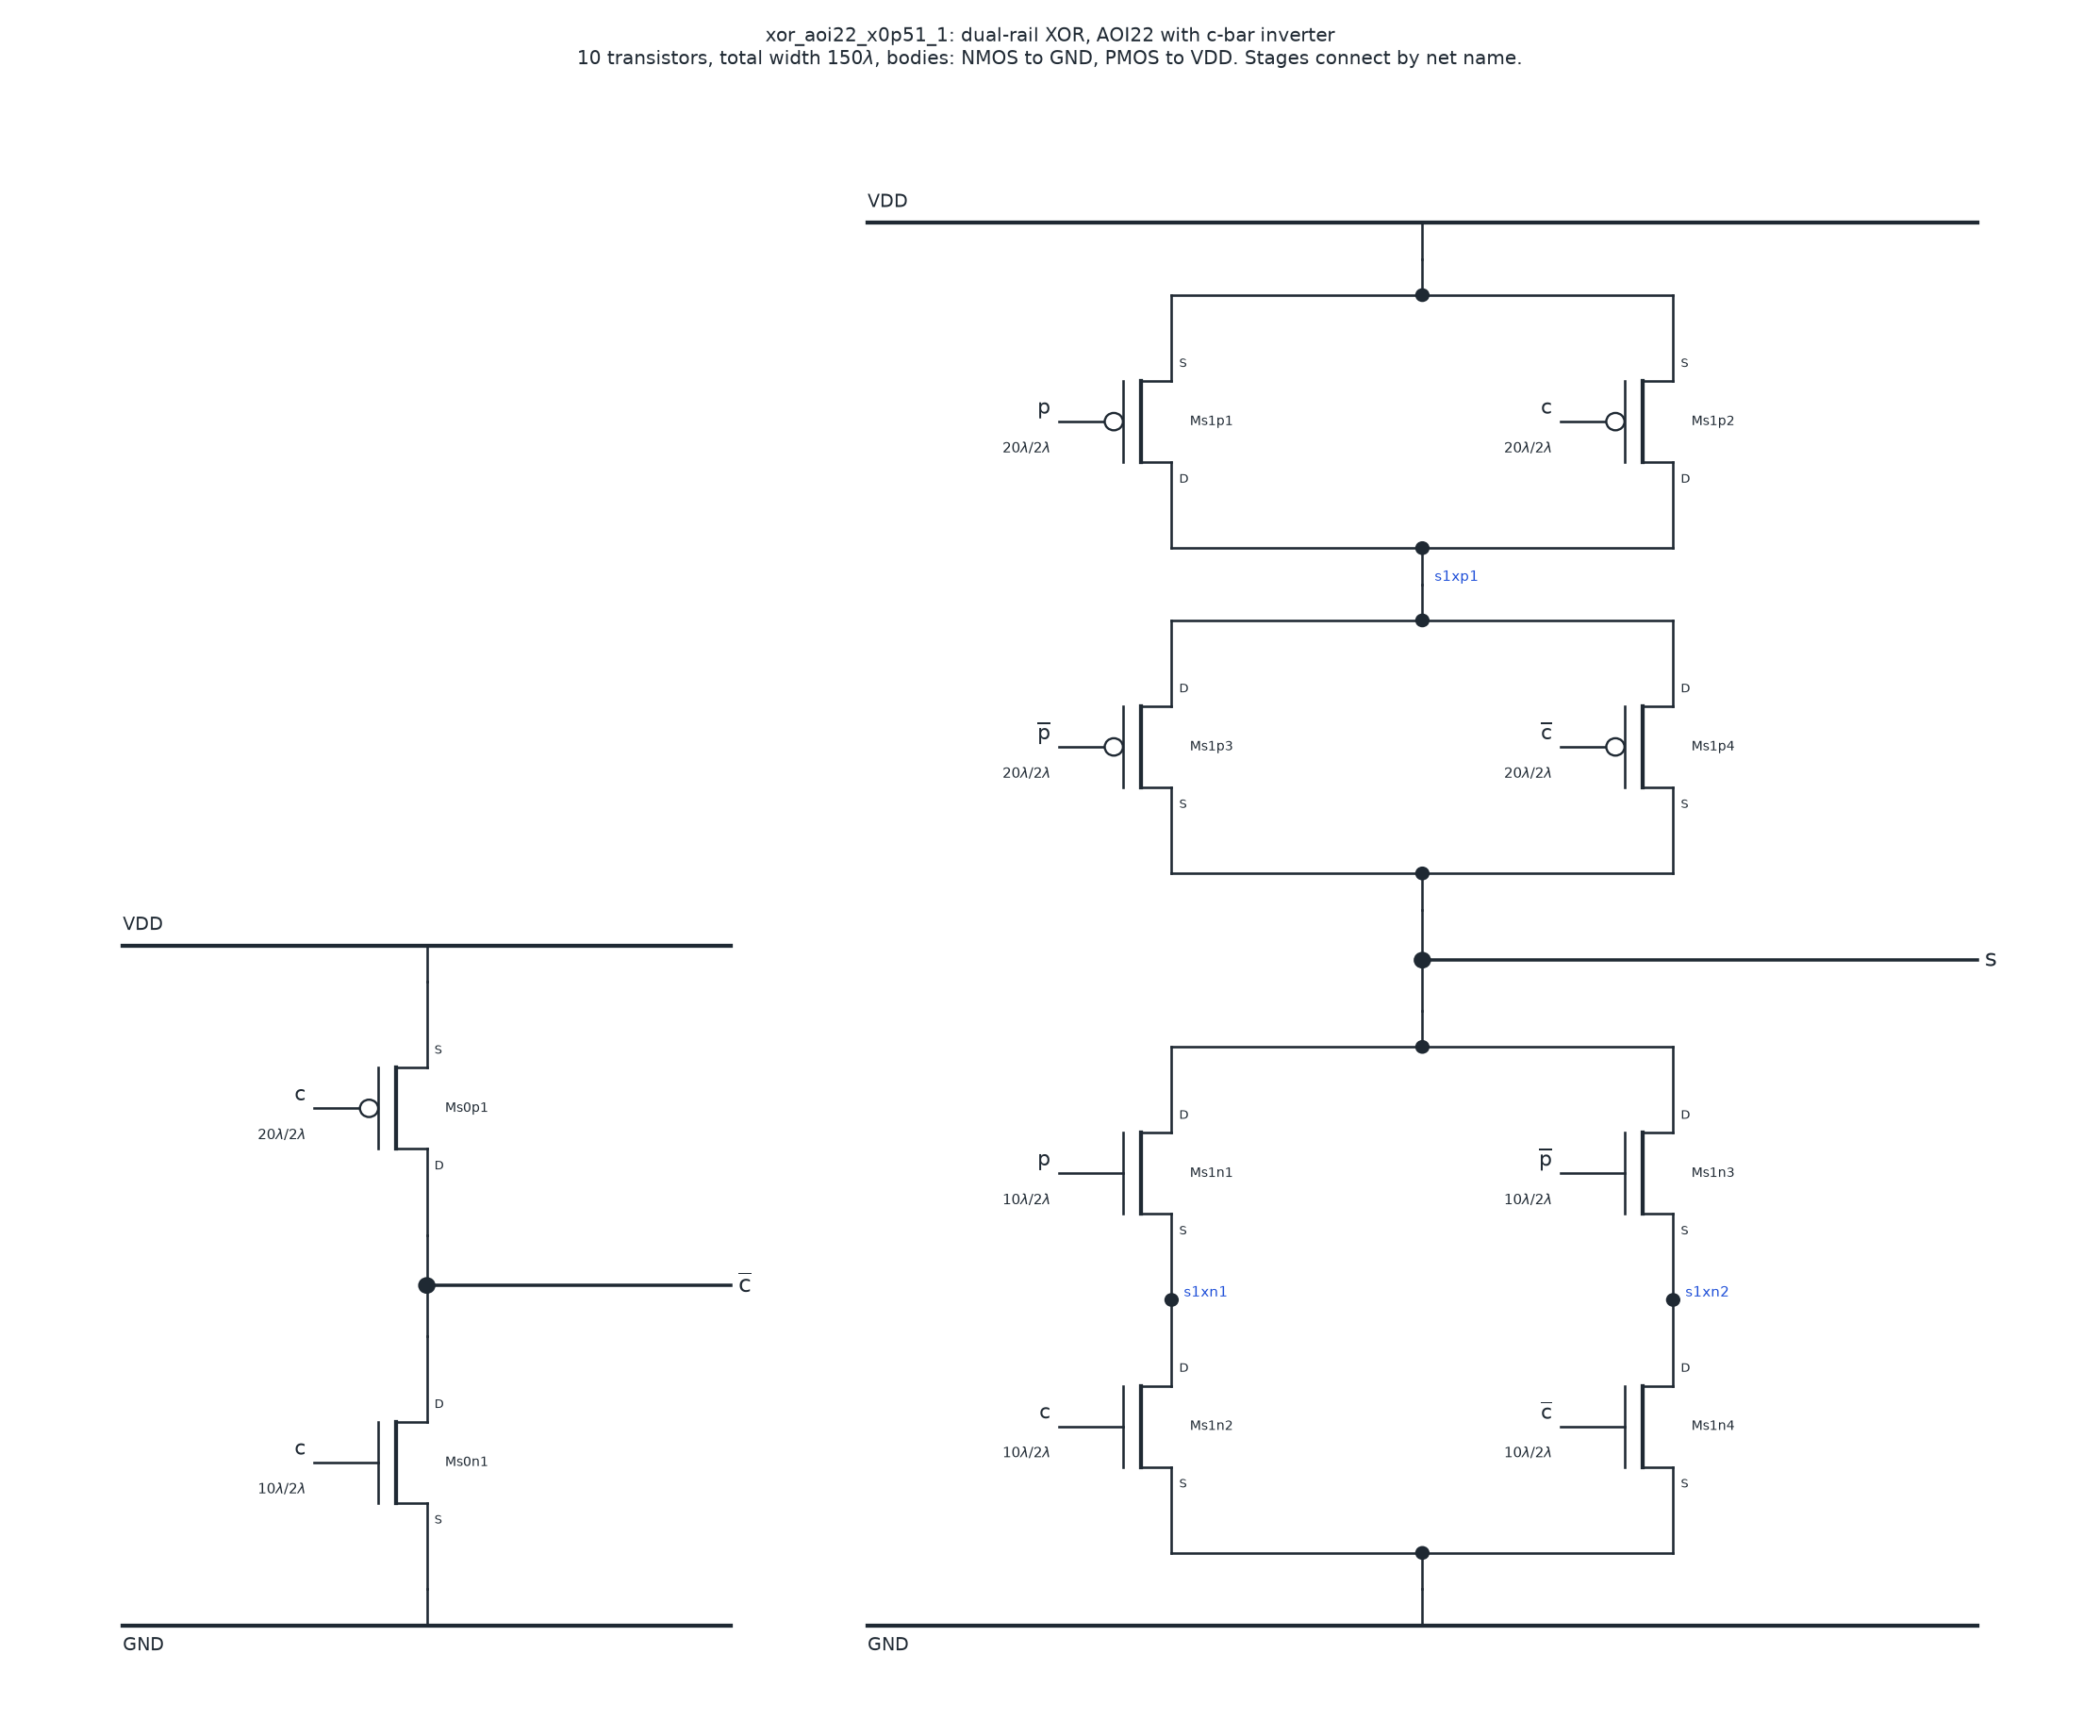
\includegraphics[width=0.48\textwidth]{figures/../../schematics/transistor_level/final/xor_aoi22_x0p51_1.png}\caption{Dual-rail XOR for S3 with c-bar inverter (xor\_aoi22\_x0p51\_1).}\end{figure}
\begin{figure}[H]\centering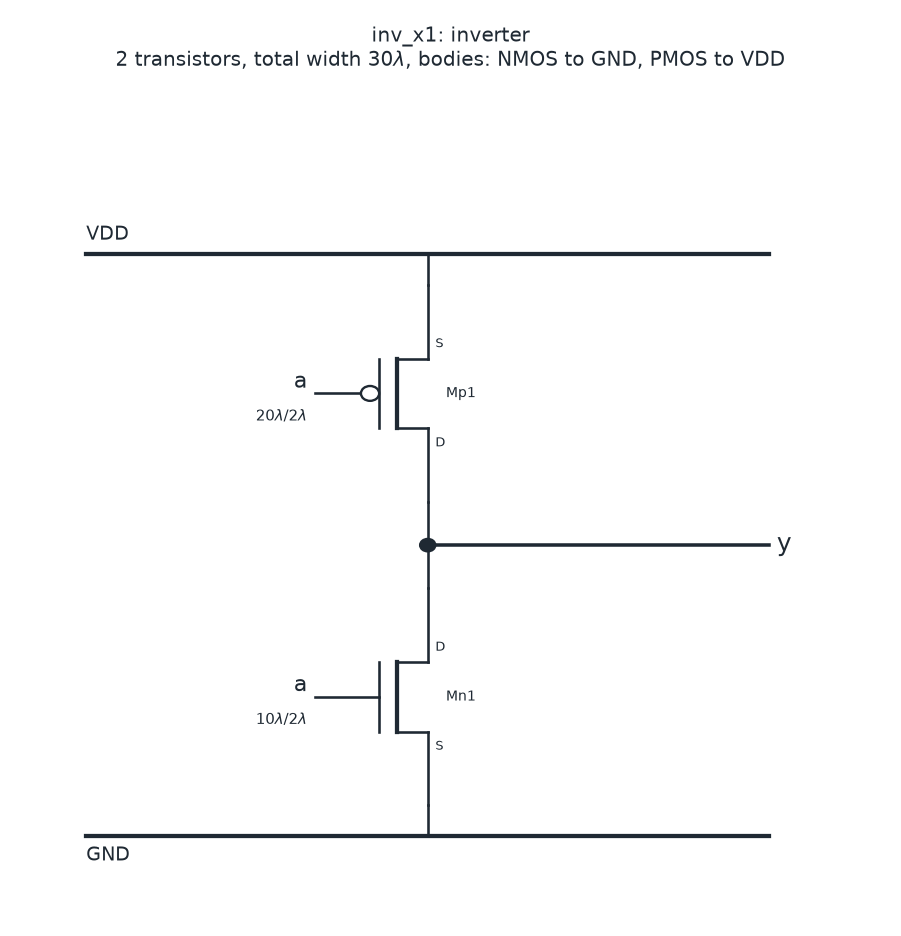
\includegraphics[width=0.48\textwidth]{figures/../../schematics/transistor_level/final/inv_x1.png}\caption{C0 inverter (inv\_x1).}\end{figure}


\subsection{D flip-flop}
TSPC and a static transmission-gate master-slave flip-flop were compared with a 15 fF load: TSPC 172.9 ps clock-to-Q and 40.0 ps setup; master-slave 200.8 ps and 116.0 ps. TSPC is about 100 ps better on clock-to-Q plus setup, with 11 transistors against 22. The course formula alone slightly favours the master-slave because of its negative hold time, but it would give a slower clock in practice, so TSPC was chosen. TSPC nodes are dynamic, so it needs a minimum clock frequency; this was not characterised.

Stage drives are $\times$0.6, $\times$1.0, $\times$1.0, $\times$2.0, found by search at the largest adder pin load, 47.8 fF including wire.

\begin{figure}[H]\centering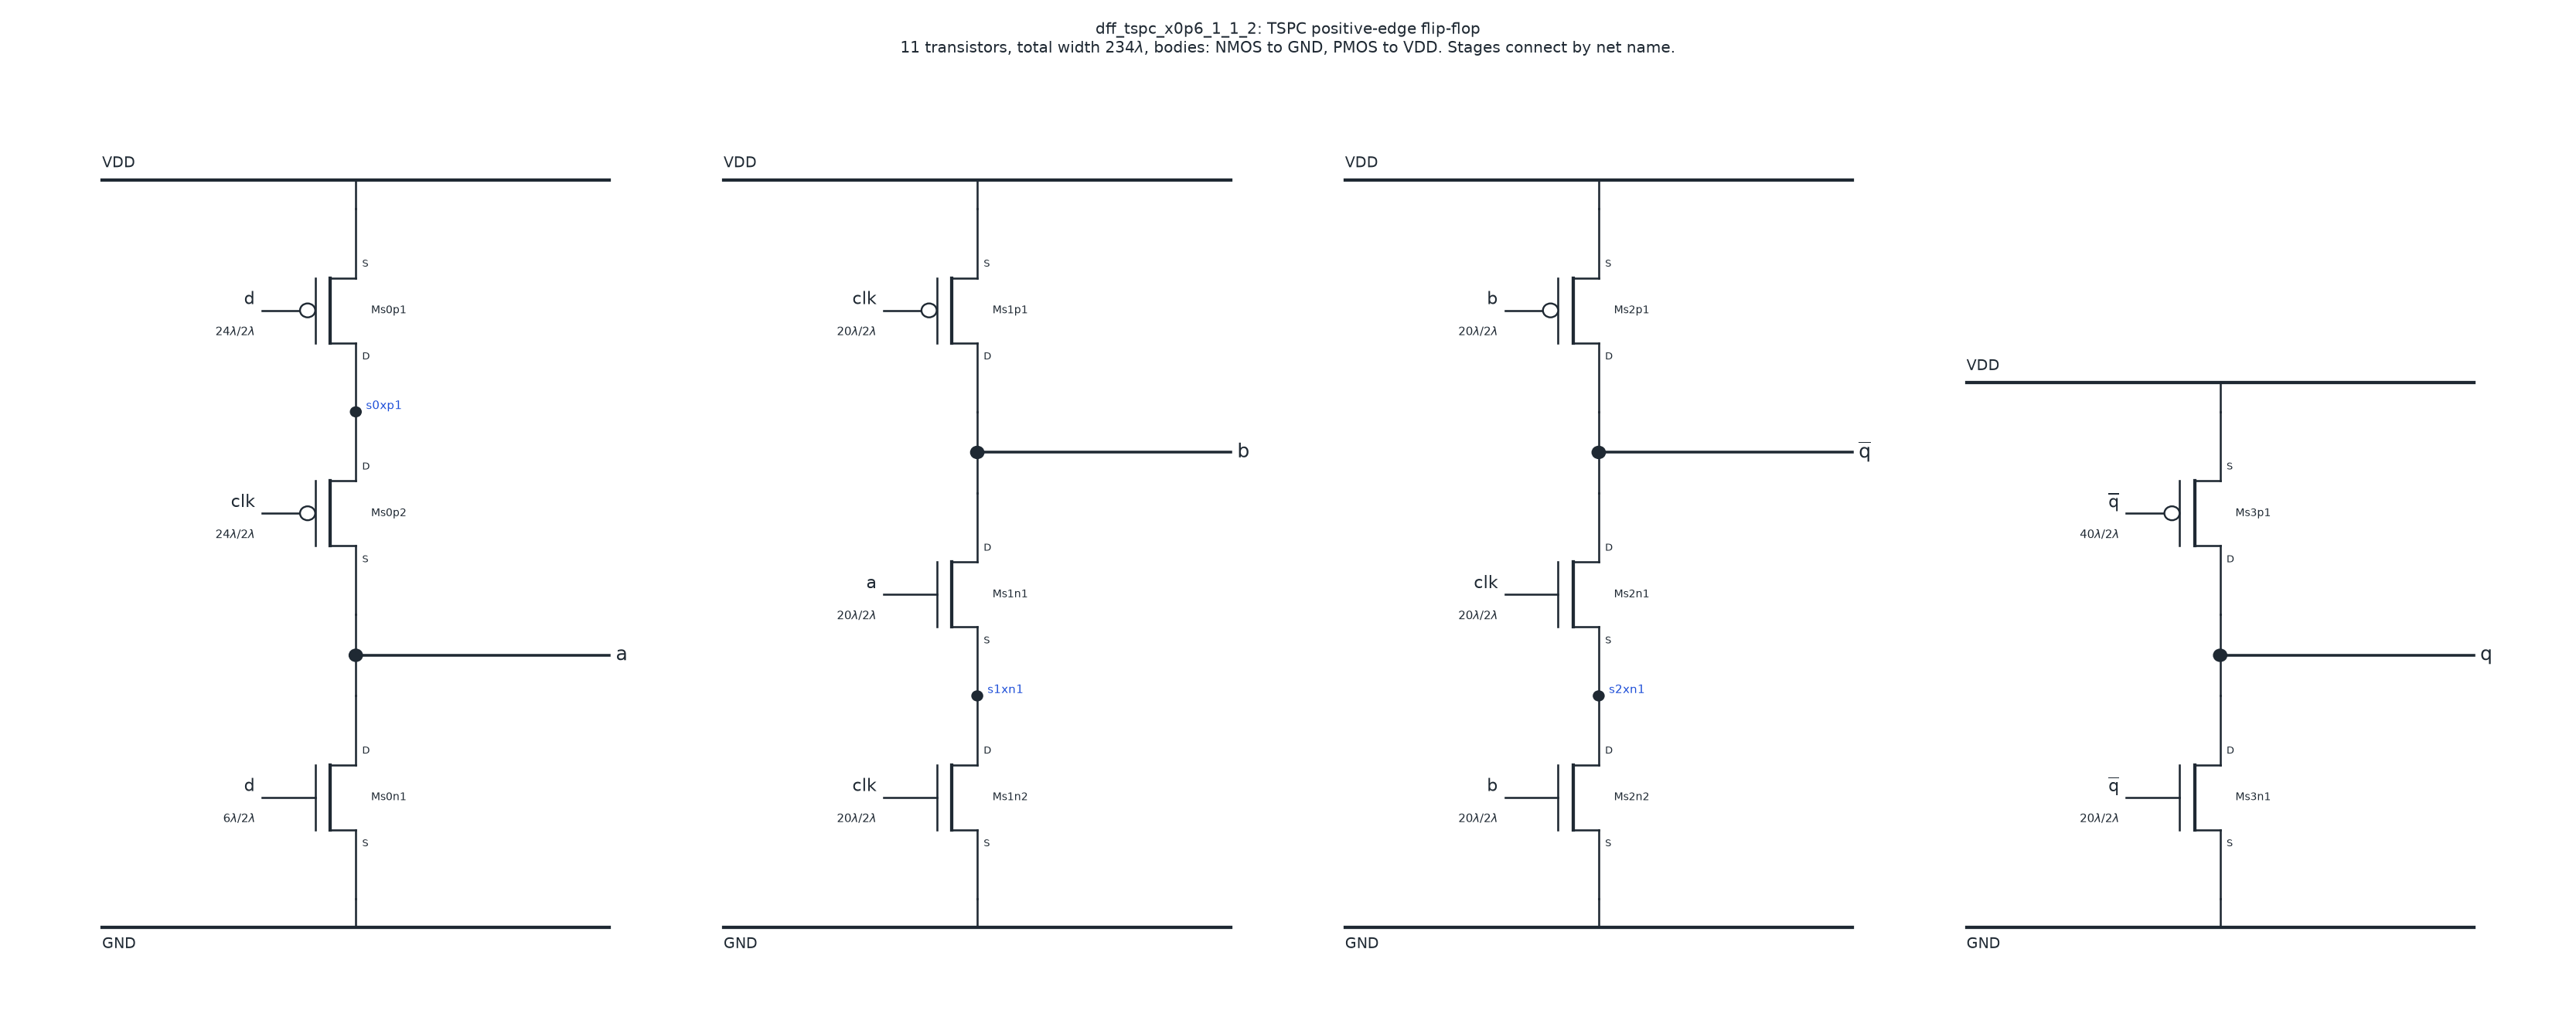
\includegraphics[width=\textwidth]{figures/../../schematics/transistor_level/final/dff_final.png}\caption{Final TSPC flip-flop.}\end{figure}

\section{Block simulation}
Every cell and block was exhaustively simulated at transistor level through finite inverter drivers, with the 20$\lambda$/10$\lambda$ inverter on each output, in binary and in shuffled order. A DC solution for every vector checks for static current. The unit-size 5-high $C_4$ gate, used only by the rejected candidate C2, needed 3 ns per vector to settle within 10\% of VDD (1.604 V at 980 ps), so its row uses 3 ns; all others use 1 ns.

\begin{table}[H]\centering
\small
\caption{Truth-table results, library at unit size}
\begin{tabular}{rrrrr}
\toprule
\textbf{Cells and blocks} & \textbf{Failing} & \textbf{Worst VOH (V)} & \textbf{Worst VOL (V)} & \textbf{Largest DC current (nA)} \\
\midrule
30 & 0 & 1.7289 & 0.0113 & 0.72 \\
\bottomrule
\end{tabular}
\end{table}

\begin{figure}[H]\centering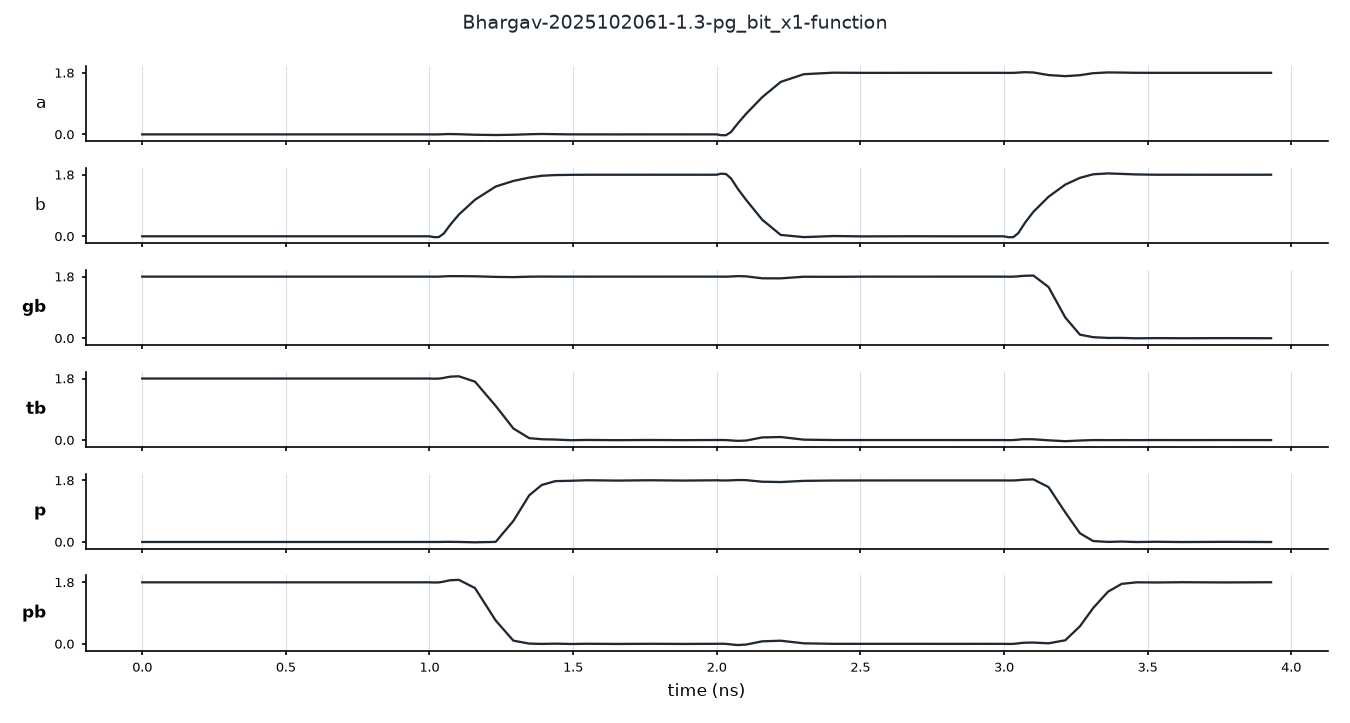
\includegraphics[width=0.9\textwidth]{figures/wave_pg.png}\caption{P/G bit waveforms.}\end{figure}
\begin{figure}[H]\centering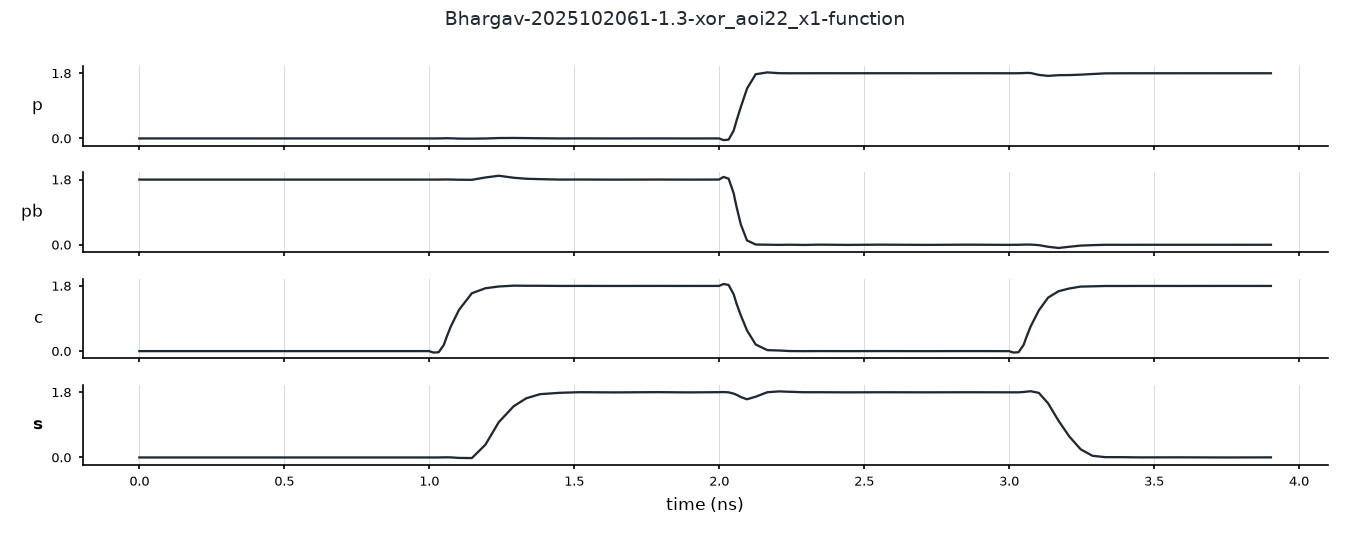
\includegraphics[width=0.9\textwidth]{figures/wave_xor.png}\caption{Dual-rail XOR waveforms.}\end{figure}

\noindent Final adder, all 512 input combinations, each twice: schematic 0 errors, extracted 0 errors.

\section{Flip-flop characterisation}
Measured at 50\% VDD. $t_{cq}$ is with data well before the clock. $t_{setup}$ is the shortest D-to-clock time keeping clock-to-Q within 10\% of $t_{cq}$. $t_{hold}$ is the shortest clock-to-D time for which a later data change leaves Q correct, with no disturbance above 10\% of VDD. Both data values were tested and the larger is reported. Definitions follow Stojanovi\'c and Oklobd\v{z}ija~\cite{stoj}.

\begin{table}[H]\centering
\small
\caption{Flip-flop timing at 47.8 fF load}
\begin{tabular}{lrr}
\toprule
\textbf{Quantity (ps)} & \textbf{Schematic} & \textbf{Post-layout} \\
\midrule
Clock to Q, Q rising & 134.1 & 136.1 \\
Clock to Q, Q falling & 208.5 & 204.2 \\
Setup, D rising & -26.0 & -8.0 \\
Setup, D falling & 34.0 & 38.0 \\
Hold, D rising & -11.7 & -11.7 \\
Hold, D falling & 55.1 & 45.7 \\
Worst tcq / tsetup / thold & 208.5 / 34.0 / 55.1 & 204.2 / 38.0 / 45.7 \\
\bottomrule
\end{tabular}
\end{table}

\begin{figure}[H]\centering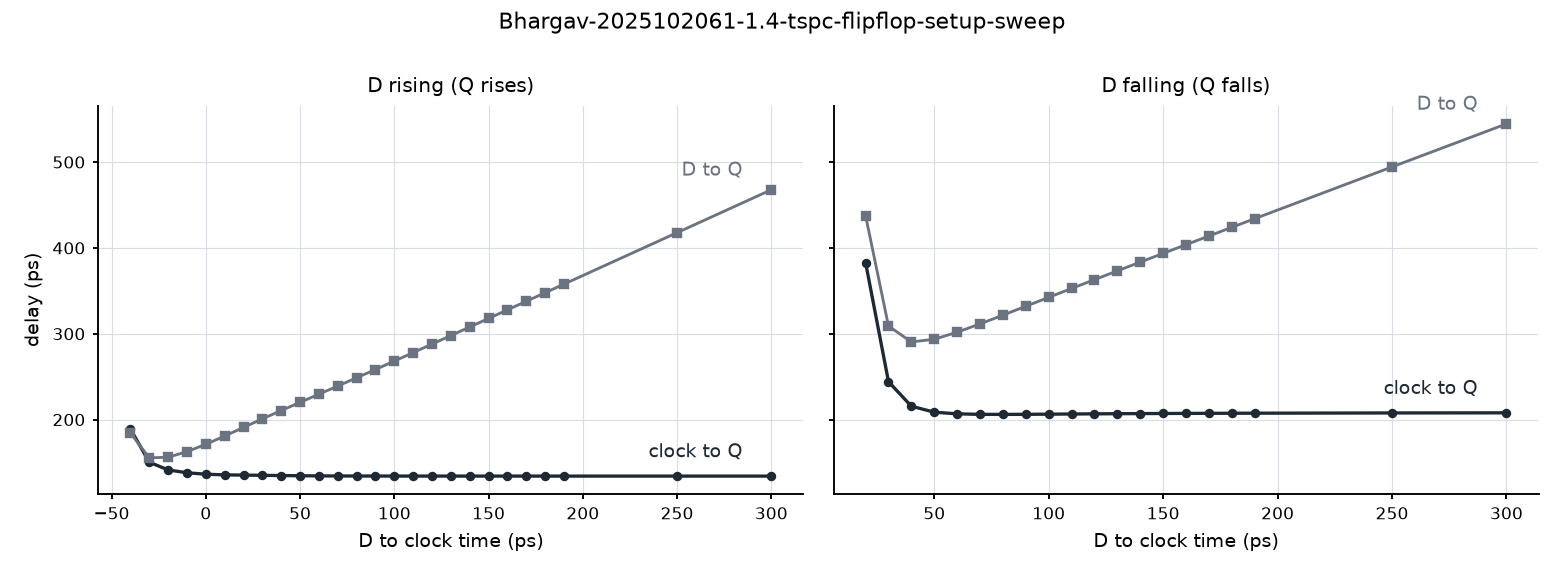
\includegraphics[width=0.95\textwidth]{figures/dff_sweep.png}\caption{Delay against D-to-clock time, schematic.}\end{figure}

\section{Block layouts}
Layouts were made in MAGIC with the provided technology file. Every cell passes DRC with zero errors, and each extracted netlist matches the schematic in LVS, with parallel fingers merged.

\begin{table}[H]\centering
\footnotesize
\caption{Each block: schematic against extracted, worst over all its single-input transitions}
\resizebox{\textwidth}{!}{
\begin{tabular}{lrrrrrrrrr}
\toprule
\textbf{Block} & \textbf{T} & \textbf{W x H (lambda)} & \textbf{Area (um2)} & \textbf{DRC} & \textbf{LVS} & \textbf{Sch tpLH} & \textbf{Sch tpHL} & \textbf{Post tpLH} & \textbf{Post tpHL} \\
\midrule
pg0 & 20 & 137 x 178 & 197.5 & 0 & match & 187.21 & 168.95 & 201.02 & 176.08 \\
pg1 & 20 & 137 x 194 & 215.3 & 0 & match & 187.4 & 171.1 & 200.97 & 169.7 \\
pg2 & 20 & 137 x 166 & 184.2 & 0 & match & 195.19 & 176.14 & 206.87 & 180.24 \\
pg3 & 20 & 137 x 161 & 178.7 & 0 & match & 199.86 & 189.09 & 210.24 & 190.19 \\
carry & 74 & 525 x 223 & 948.3 & 0 & match & 319.87 & 306.42 & 335.79 & 336.37 \\
sum0 & 10 & 84 x 166 & 112.9 & 0 & match & 176.33 & 173.69 & 182.49 & 171.72 \\
sum1 & 10 & 84 x 151 & 102.7 & 0 & match & 157.14 & 144.1 & 161.33 & 142.78 \\
sum2 & 10 & 84 x 139 & 94.6 & 0 & match & 134.23 & 119.06 & 134.85 & 118.7 \\
sum3 & 10 & 84 x 121 & 82.3 & 0 & match & 134.71 & 114.42 & 137.22 & 117.54 \\
\bottomrule
\end{tabular}
}
\end{table}

\begin{table}[H]\centering
\small
\caption{Flip-flop layout}
\begin{tabular}{rrrr}
\toprule
\textbf{Width x height (lambda)} & \textbf{Area (um2)} & \textbf{DRC} & \textbf{LVS} \\
\midrule
99 x 142 & 113.9 & 0 & match \\
\bottomrule
\end{tabular}
\end{table}

The layout figures below are screenshots of MAGIC's own layout window, taken with the cell loaded and fitted to the window.

\begin{figure}[H]\centering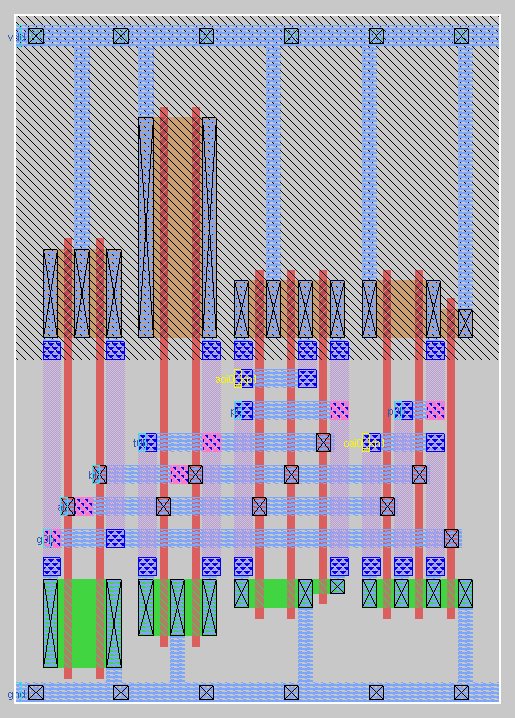
\includegraphics[width=0.62\textwidth]{figures/magic_pg.png}\caption{P/G bit 0 tile in MAGIC, as placed in the final adder.}\end{figure}
\begin{figure}[H]\centering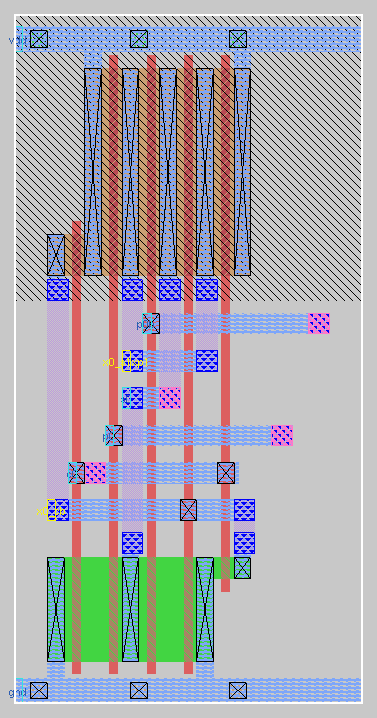
\includegraphics[width=0.62\textwidth]{figures/magic_sum.png}\caption{Sum bit 0 tile in MAGIC.}\end{figure}
\begin{figure}[H]\centering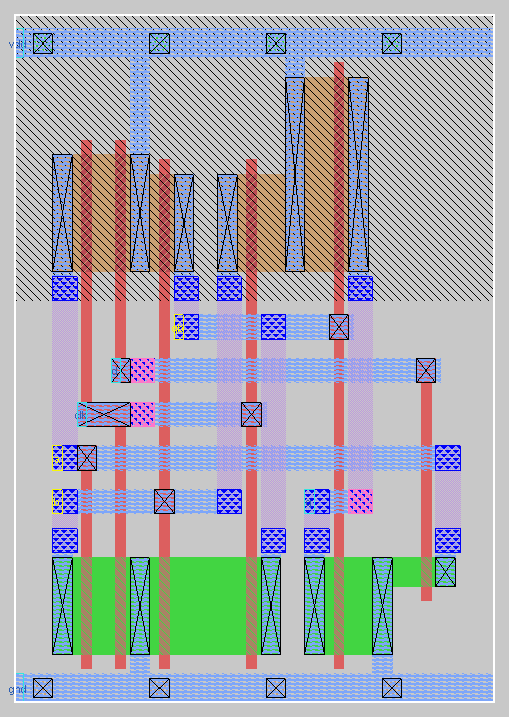
\includegraphics[width=0.62\textwidth]{figures/magic_dff.png}\caption{TSPC flip-flop layout in MAGIC.}\end{figure}
\begin{figure}[H]\centering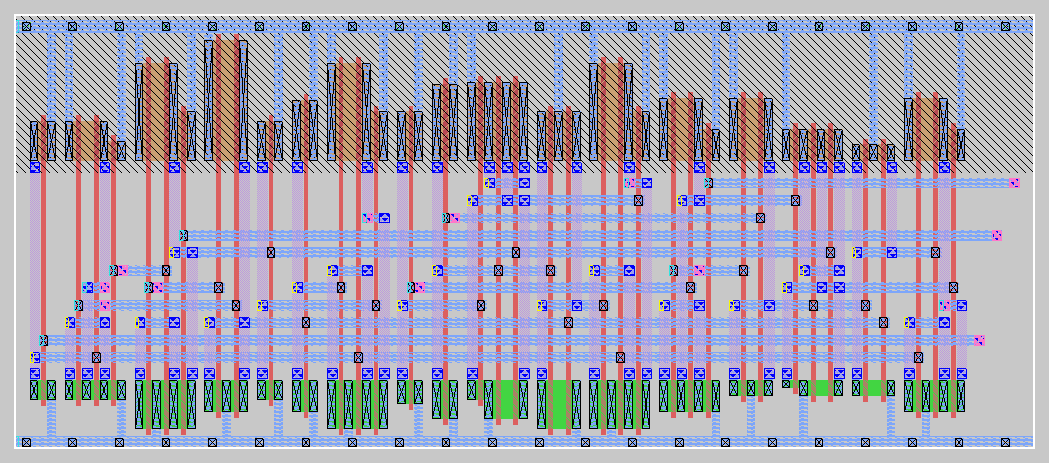
\includegraphics[width=0.95\textwidth]{figures/magic_carry.png}\caption{Carry block tile in MAGIC.}\end{figure}

\section{Integration}
The complete circuit of Figure 1(i) has 9 input flip-flops, the adder and 5 output flip-flops. It was simulated with the hint vector, the 30 slowest arcs from the adder search, and 200 random vectors. A vector captured at one rising edge must appear at the output flip-flops after the next. The limit below is the shortest clock period, found by binary search to 5 ps, with zero wrong samples.

\begin{table}[H]\centering
\small
\caption{Registered system}
\begin{tabular}{lrr}
\toprule
\textbf{Quantity} & \textbf{Schematic} & \textbf{Post-layout} \\
\midrule
Vectors checked & 264 & 264 \\
Shortest working period (ps) & 740.2 & 872.1 \\
Maximum verified frequency (GHz) & 1.3509 & 1.1467 \\
Wrong samples at that period & 0 & 0 \\
\bottomrule
\end{tabular}
\end{table}

\begin{figure}[H]\centering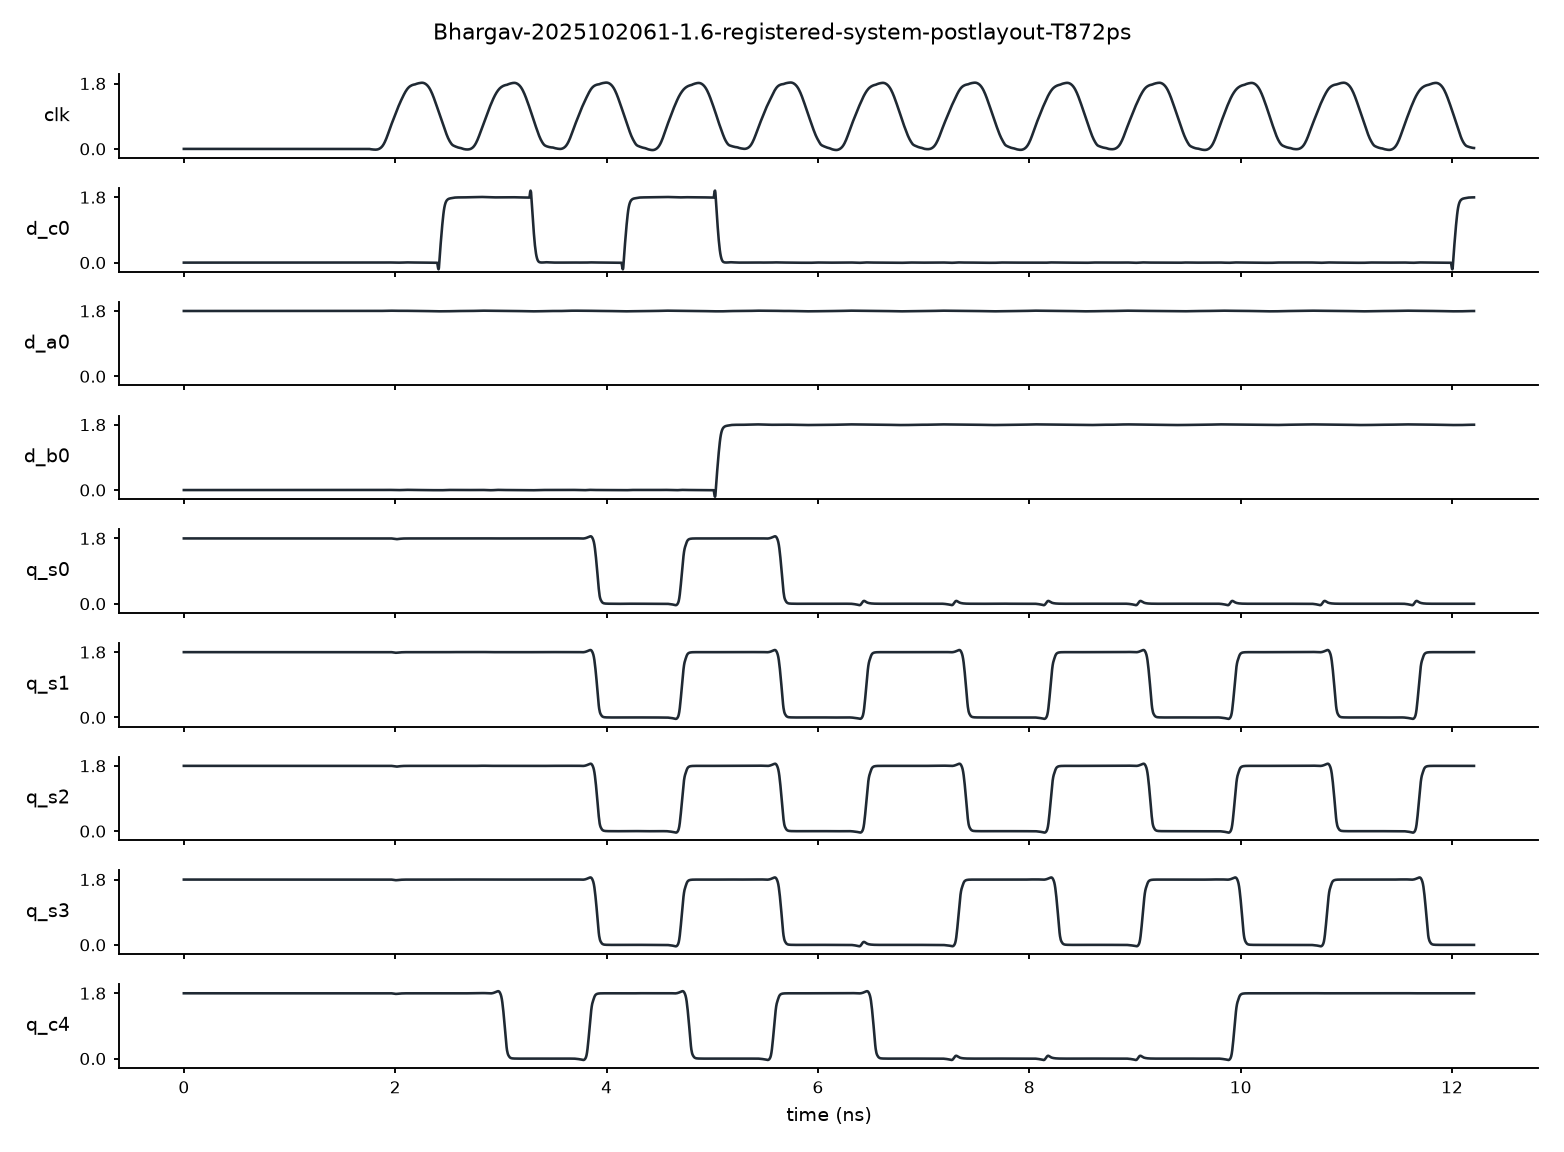
\includegraphics[width=\textwidth]{figures/system_postlayout.png}\caption{Extracted registered circuit at the verified limit, first vectors. Q values follow inputs after one clock period.}\end{figure}

\section{Floor plan and pitches}
\begin{figure}[H]\centering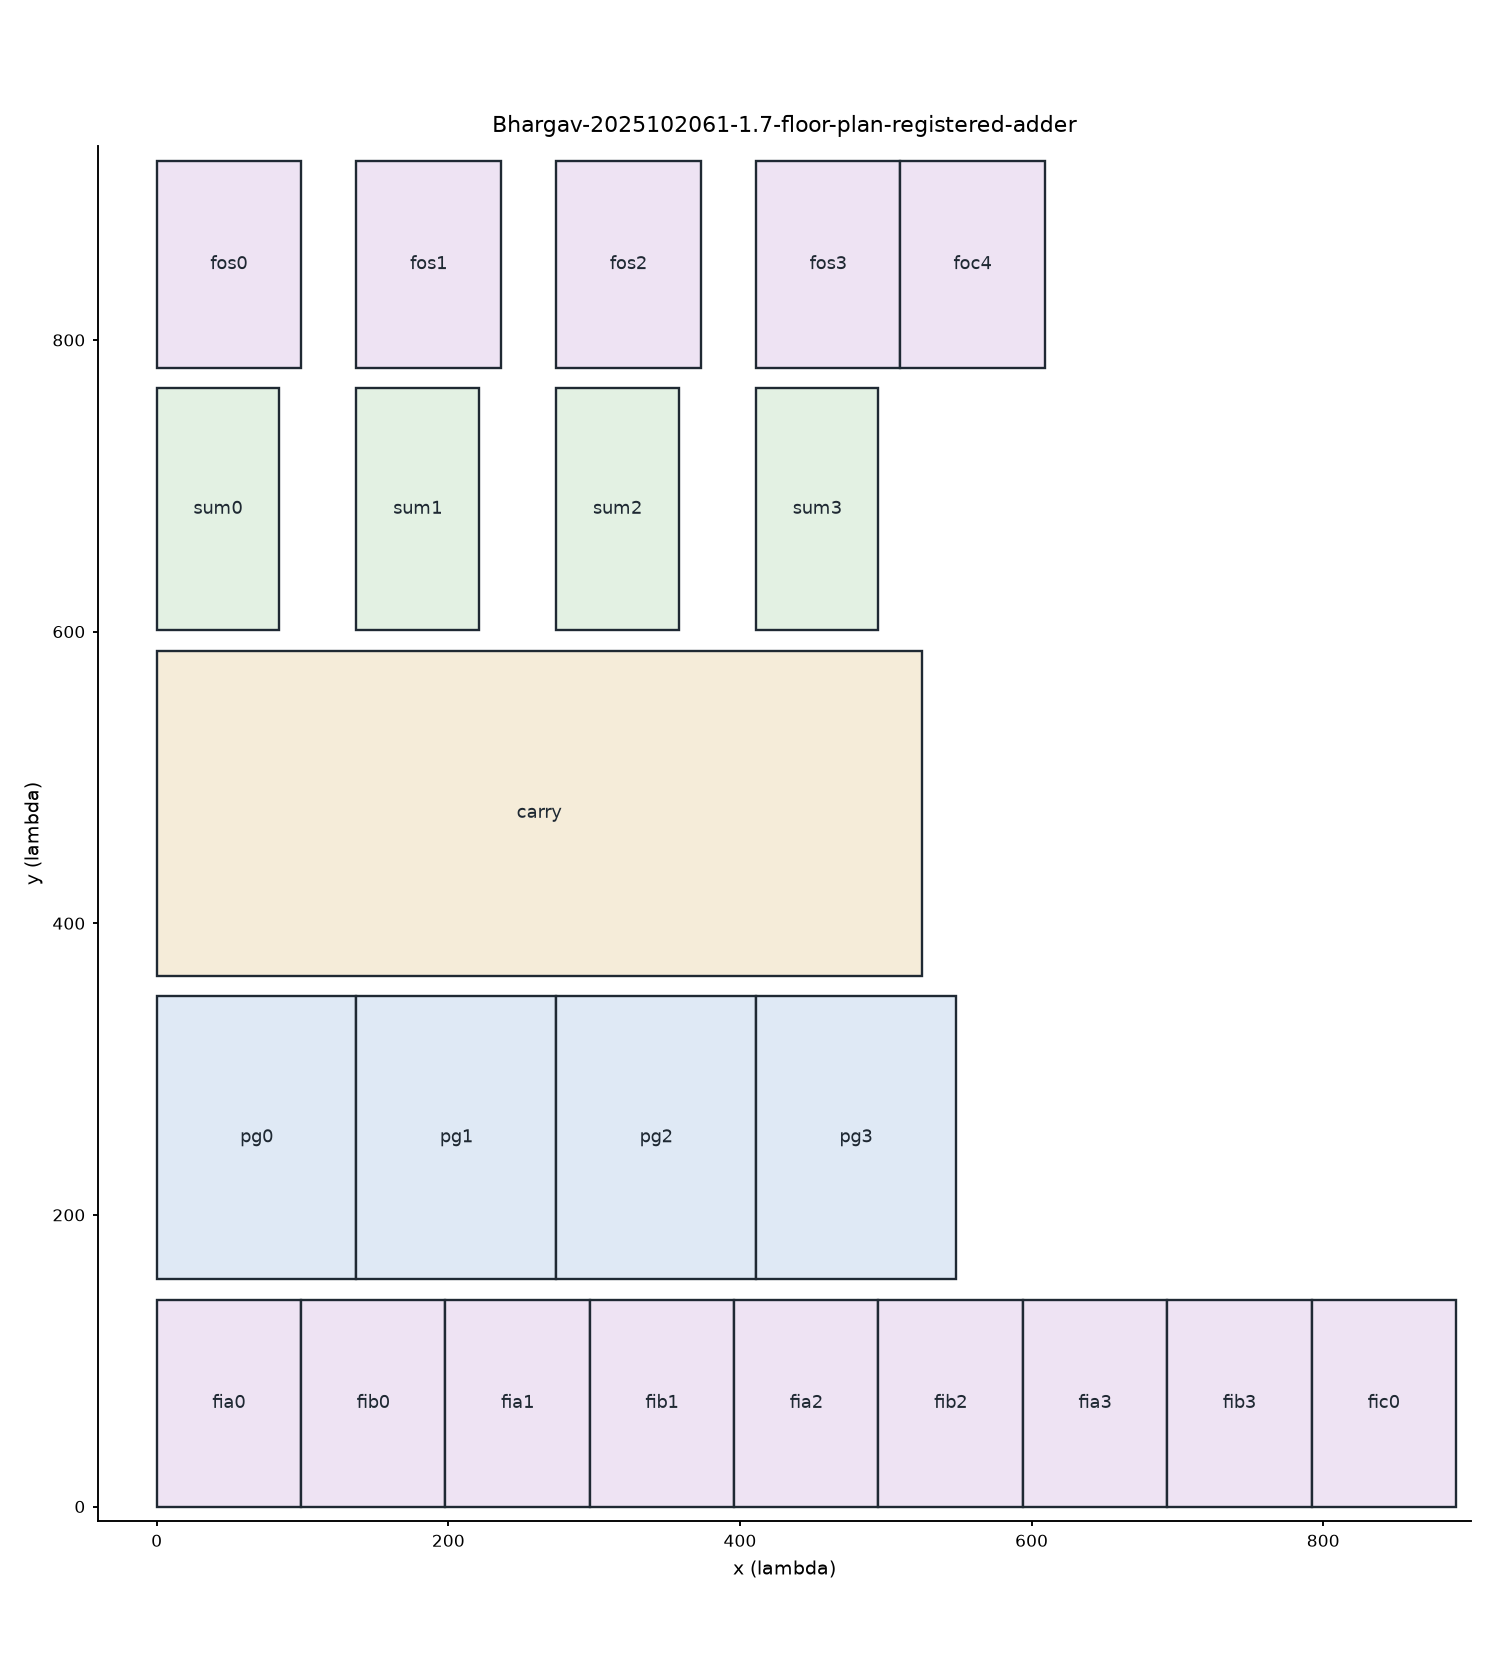
\includegraphics[width=0.82\textwidth]{figures/floorplan.png}\caption{Floor plan of the registered adder. Rows from bottom: input flip-flops, P/G bits, carry block, sum bits, output flip-flops.}\end{figure}

The P/G bit cells form the regular structure, and sum cells align to their columns.

\begin{table}[H]\centering
\small
\caption{Pitches}
\begin{tabular}{lrr}
\toprule
\textbf{Structure} & \textbf{Pitch (lambda)} & \textbf{Pitch (um)} \\
\midrule
Horizontal: bit pitch, P/G and sum columns & 137 & 12.33 \\
Horizontal: flip-flop cell & 99 & 8.91 \\
Vertical: row pitches, bottom to top & 156, 208, 237, 180 & 14.04, 18.72, 21.33, 16.20 \\
Channel track pitch, metal 1 & 9 & 0.81 \\
Gate pitch, shared / contacted diffusion & 7 / 9 & 0.63 / 0.81 \\
Over-cell routing grid, metal 3 and 4 & 9 & 0.81 \\
\bottomrule
\end{tabular}
\end{table}

\section{Full layout: schematic against post-layout}
Adder layout: DRC 0, LVS match: 194 merged devices, 108 nets, 712 extracted capacitors totalling 376.9 fF. Registered layout: DRC 0, LVS match: 348 merged devices, 207 nets, area 7005.5 $\mu$m$^2$.

\begin{figure}[H]\centering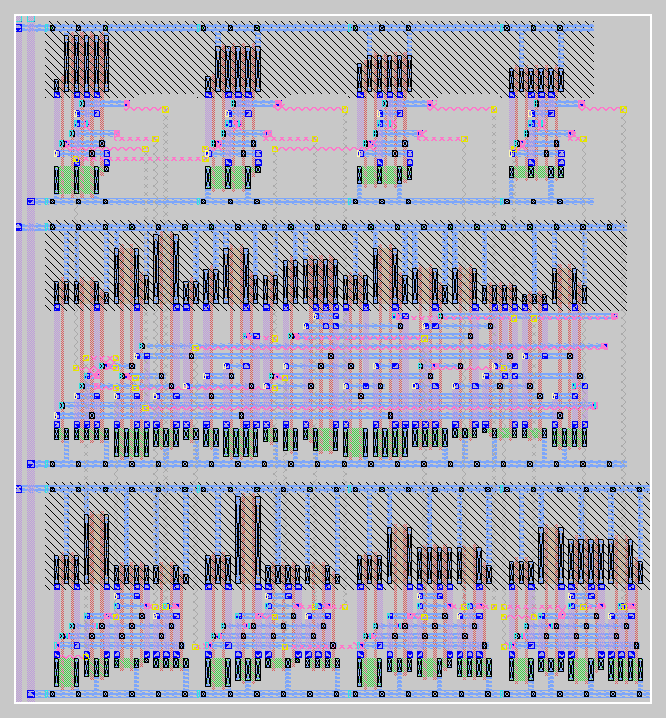
\includegraphics[width=0.92\textwidth]{figures/magic_adder.png}\caption{Final 4-bit adder layout in MAGIC: P/G row at the bottom, carry block, sum row at the top.}\end{figure}
\begin{figure}[H]\centering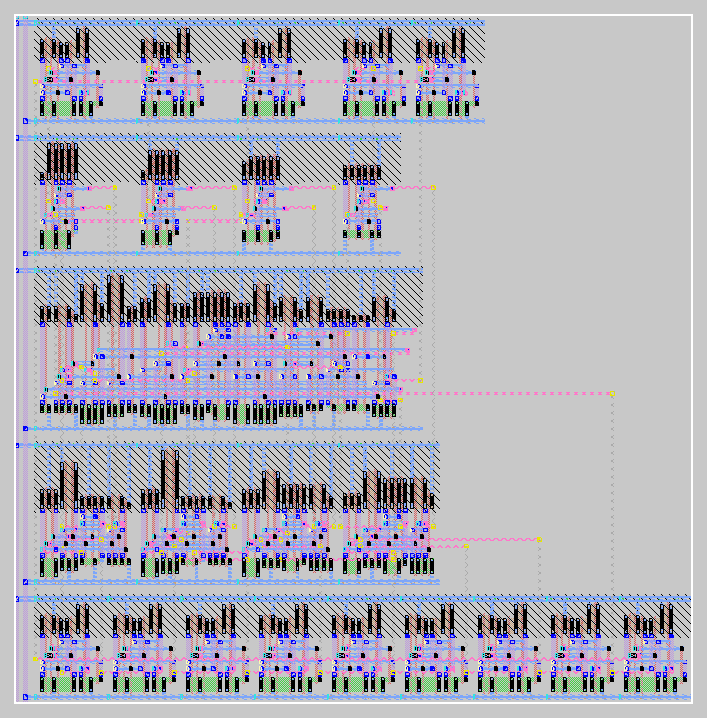
\includegraphics[width=0.85\textwidth]{figures/magic_registered.png}\caption{Registered adder layout in MAGIC: input flip-flops at the bottom, output flip-flops at the top.}\end{figure}

\begin{table}[H]\centering
\footnotesize
\caption{Worst delay per output, all single-input transitions (ps)}
\begin{tabular}{llrrr}
\toprule
\textbf{Output} & \textbf{Edge} & \textbf{Schematic} & \textbf{Post-layout} & \textbf{Change (\%)} \\
\midrule
S0 & tpLH & 349.7 & 387.1 & 10.7 \\
S0 & tpHL & 352.7 & 394.8 & 11.9 \\
S1 & tpLH & 429.9 & 536.9 & 24.9 \\
S1 & tpHL & 409.2 & 508.1 & 24.2 \\
S2 & tpLH & 499.7 & 562.8 & 12.6 \\
S2 & tpHL & 470.1 & 543.6 & 15.6 \\
S3 & tpLH & 516.3 & 579.9 & 12.3 \\
S3 & tpHL & 491.1 & 570.2 & 16.1 \\
C4 & tpLH & 414.2 & 490.4 & 18.4 \\
C4 & tpHL & 399.2 & 466.4 & 16.9 \\
\bottomrule
\end{tabular}
\end{table}

Worst single-input delay rose from 516.3 to 579.9 ps (12.3\%). Note that the final sizes were tuned with wire load in mind, so the schematic column is not the best schematic result.

\section{Critical path}
\subsection{Course hint vector}
With $A=1111$, $B=0000$, toggling $C_0$ both ways gives both edges at each output. Rising $C_0$ alone gives only falling sums and rising $C_4$. All $S$ outputs flip, as the hint predicts.

\begin{table}[H]\centering
\footnotesize
\caption{Hint vector, extracted netlist}
\begin{tabular}{llll}
\toprule
\textbf{C0 edge} & \textbf{Output} & \textbf{Type} & \textbf{Delay (ps)} \\
\midrule
rise & S0 & tpHL & 72.8 \\
rise & S1 & tpHL & 446.81 \\
rise & S2 & tpHL & 402.78 \\
rise & S3 & tpHL & 396.98 \\
rise & C4 & tpLH & 300.03 \\
fall & S0 & tpLH & 102.04 \\
fall & S1 & tpLH & 454.15 \\
fall & S2 & tpLH & 385.19 \\
fall & S3 & tpLH & 385.81 \\
fall & C4 & tpHL & 283.28 \\
\bottomrule
\end{tabular}
\end{table}

\begin{figure}[H]\centering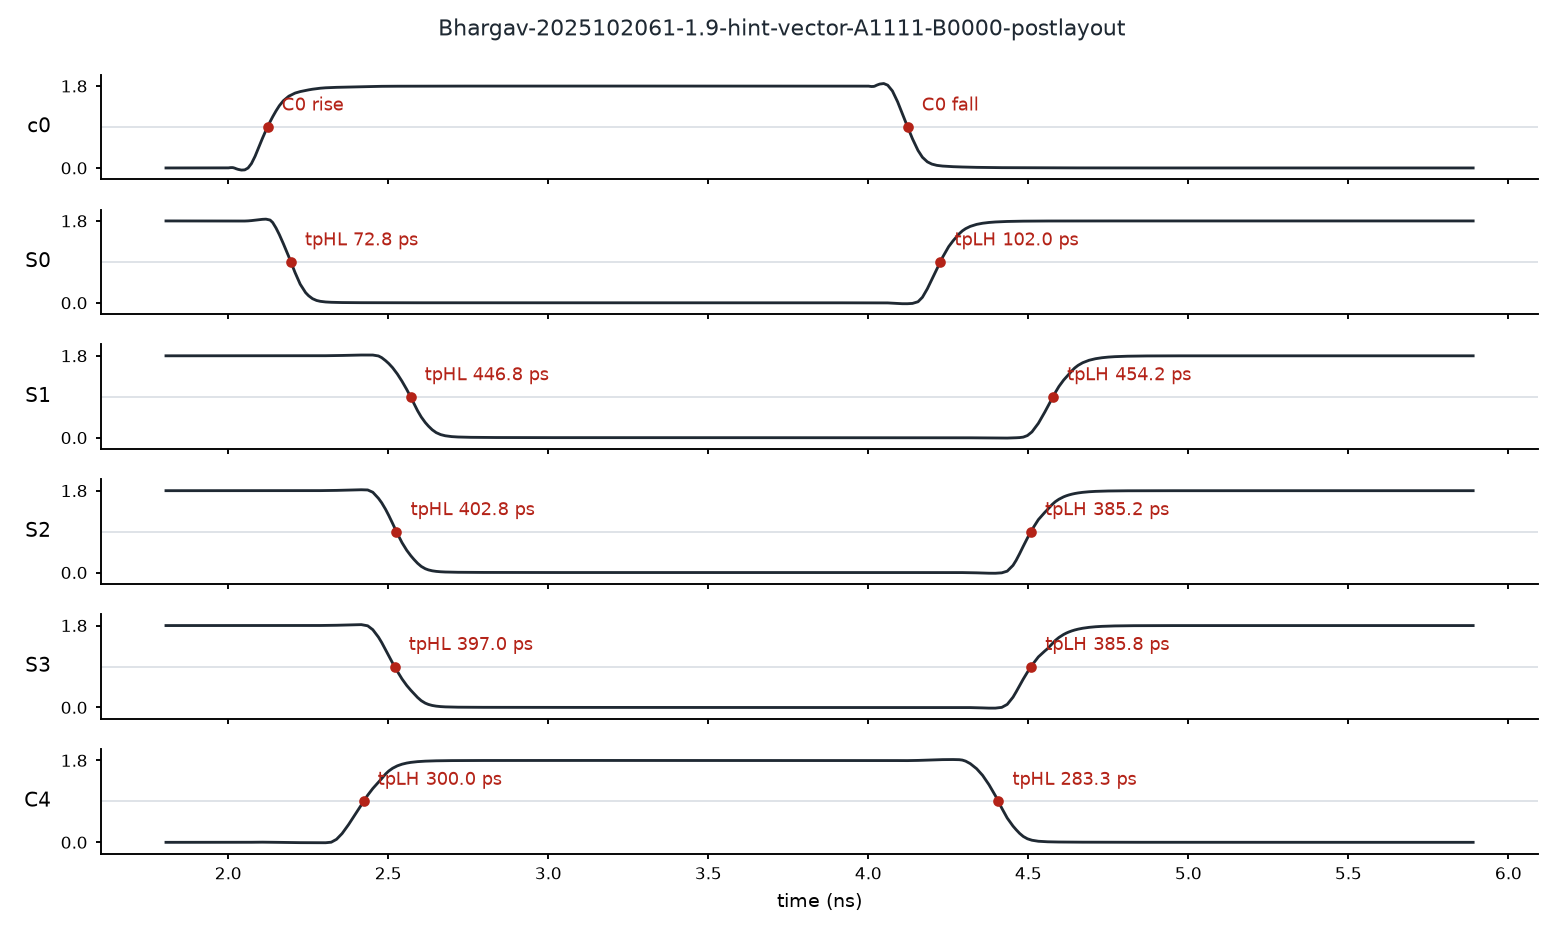
\includegraphics[width=\textwidth]{figures/hint_postlayout.png}\caption{Hint vector, extracted netlist, with 50\% crossings marked.}\end{figure}
\begin{figure}[H]\centering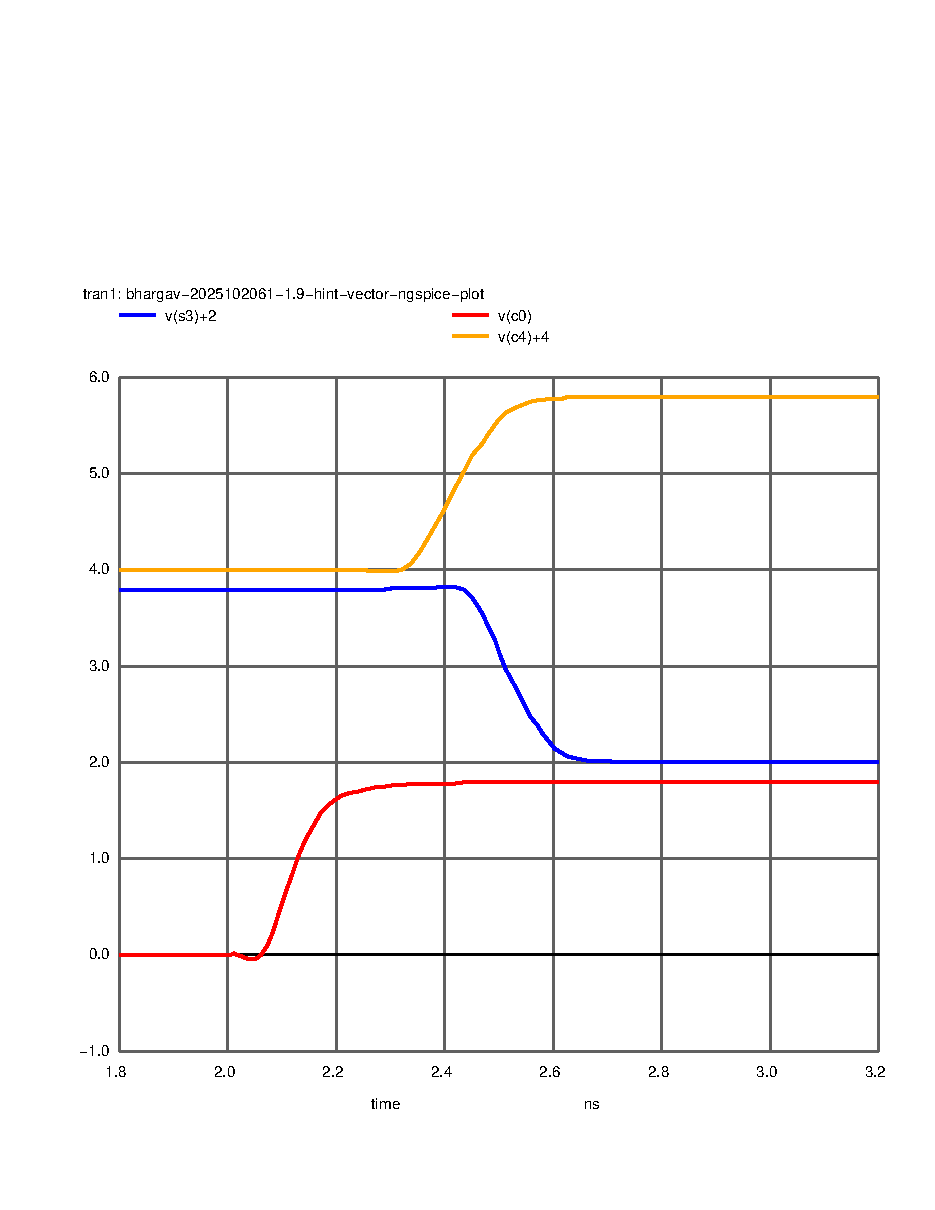
\includegraphics[width=0.7\textwidth]{figures/native_ngspice.png}\caption{The same event as drawn by ngspice itself, showing the required curplottitle. ngspice displays the title in lower case. C0, S3+2 V, C4+4 V.}\end{figure}

\subsection{True worst case}
The slowest hint-vector output is S1 at 454.1 ps, but the worst single-input transition is \textbf{a1 rise to s3 rise, A=0001 B=0101 C0=0} at \textbf{579.88 ps}. The hint vector skips the P/G stage and most of the prefix tree: $C_0$ reaches each carry through one inverter and one gate. Reporting only the hint vector would understate this design's delay by 135.7 ps.

\begin{figure}[H]\centering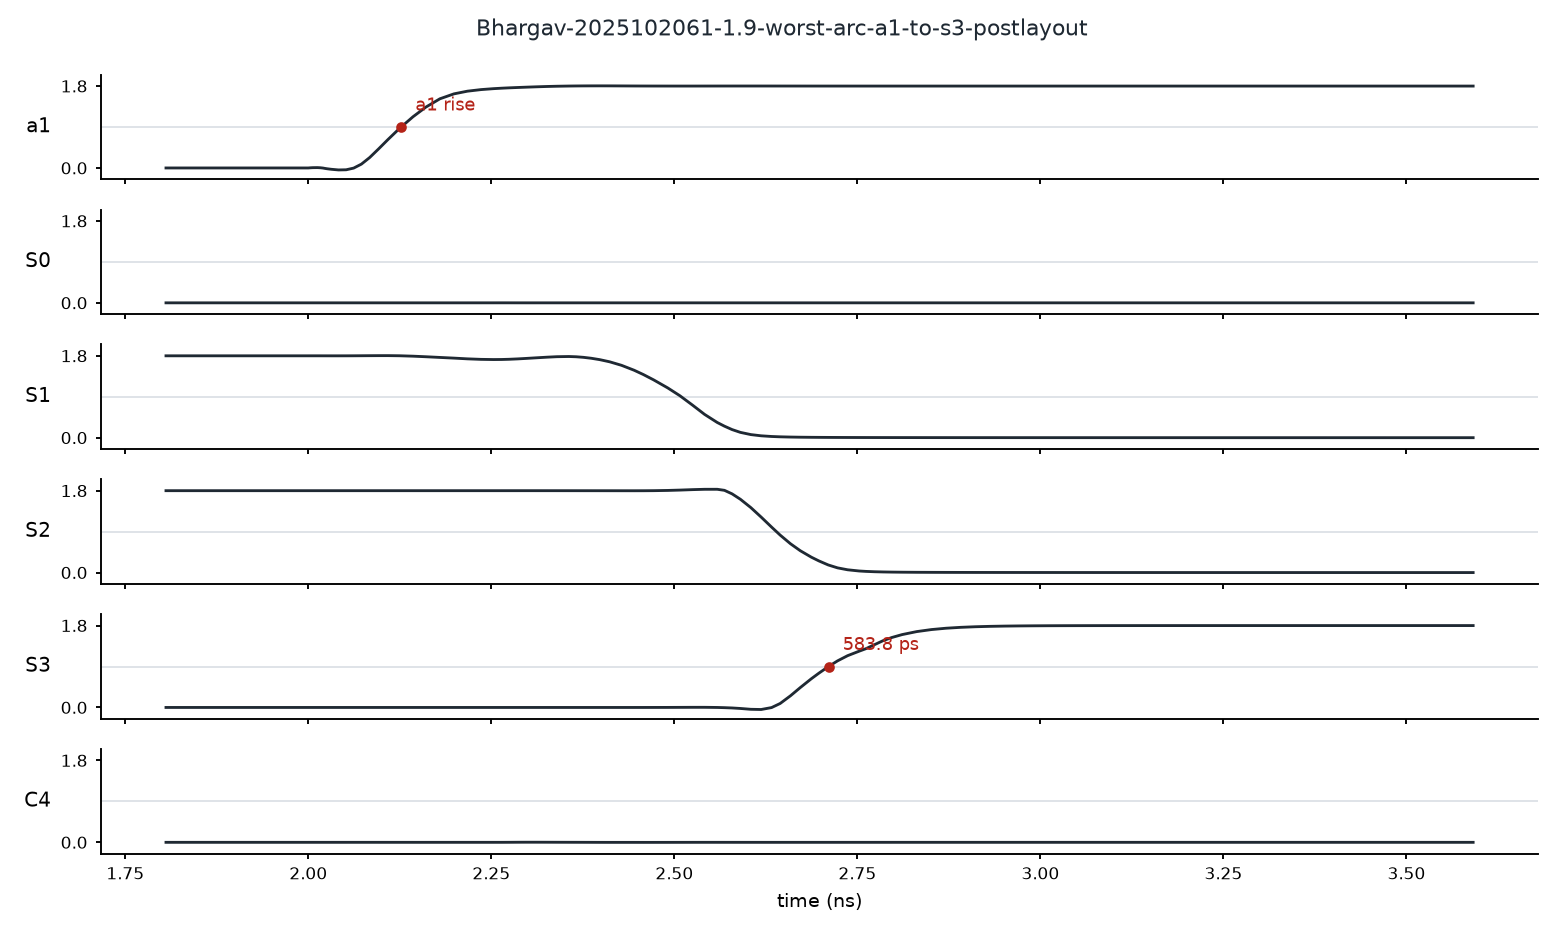
\includegraphics[width=\textwidth]{figures/worst_arc_postlayout.png}\caption{Worst single-input transition, extracted netlist.}\end{figure}

\noindent\textbf{History dependence.} Delay depends slightly on what came before. Starting this arc from a settled DC state gives 583.8 ps, against 579.88 ps inside the long all-transition walk. For the hint vector, the walk measured up to 455.23 ps against 454.1 ps above. The likely cause is charge left on internal stack nodes, which was not investigated further. Differences of this size should be read as the precision of these numbers.

\subsection{Several inputs changing together}
Registers launch all inputs together, so several can change at once. All pairs would be 261,632 transitions, so an evenly spread sample was run: 65520 transitions (one segment in 4), on the schematic with extracted wire load annotated. Worst 577.64 ps, with 0 errors. The 100 slowest pairs from that sample were then re-simulated on the extracted netlist: worst \textbf{589.85 ps}, from 4 inputs changing, measured from the earliest of them. This exceeds the single-input worst case, so it is taken as $t_{pd,max}$. This is a sample, not an exhaustive proof, so an unsampled transition could be slightly slower.

\section{Maximum clock frequency}
The course defines $f_{max}=1/(t_{pd,max}+t_{setup}+t_{hold})$. With post-layout values:
\[T=589.85+38.0+45.7=673.6\text{ ps},\quad f_{max}=1.4847\text{ GHz}.\]
At the course-formula period (673.6 ps) the extracted registered circuit gave 264 wrong output samples, so that frequency is \emph{not} reliable for this design. The formula leaves out clock-to-Q delay. A flip-flop launch actually needs $T\ge t_{cq}+t_{pd,max}+t_{setup}=204.2+589.85+38.0=832.0$ ps, or 1.2019 GHz. Simulation of the extracted circuit finds the actual limit: \textbf{1.1467 GHz} (T = 872.1 ps). The value to rely on is the simulated limit.

\section{Power}
$P_{avg}=\frac{V_{DD}}{T_2-T_1}\int_{T_1}^{T_2}I_{VDD}(t)\,dt$ for the extracted registered circuit, at the verified limit of 872.1 ps. Input drivers, clock buffers and output load inverters use a separate supply, so they are not included; the load's capacitance is still driven by the circuit. $T_1$ follows one settling cycle.

\begin{table}[H]\centering
\footnotesize
\caption{Post-layout power, with PDP = Pavg x tpd,max}
\begin{tabular}{lrrrrr}
\toprule
\textbf{Activity} & \textbf{Cycles} & \textbf{Errors} & \textbf{Pavg (mW)} & \textbf{Energy/cycle (pJ)} & \textbf{PDP (fJ)} \\
\midrule
200 random plus critical vectors & 264 & 0 & 3.3899 & 2.956 & 1999.51 \\
Hint vector, C0 toggling each cycle & 80 & 0 & 2.4954 & 2.176 & 1471.94 \\
Inputs constant (clock and flip-flops) & 40 & 0 & 0.8874 & 0.774 & 523.45 \\
\bottomrule
\end{tabular}
\end{table}

The first row is the main result. It is measured at the verified limit, not the course-formula frequency, because the circuit must run correctly for the number to mean anything.

\section{Layout resistance}\label{sec:res}
MAGIC's extraction here gives capacitance only, and its \texttt{extresist} command crashes on this layout (segmentation fault; log kept). As a substitute, the longest poly run from a contact to a gate end was measured from the layout: 152 $\lambda$, or 585.2 $\Omega$ at the technology file's 7.7 $\Omega$/square. That resistance was placed in series with \emph{every} one of the 194 gates, which is far more than any real gate sees, and all transitions were simulated again: worst single-input delay 579.88 to 600.83 ps, an increase of 20.95 ps (3.61\%). Metal and vias are not included in this bound. Metal is 0.08 $\Omega$/square and vias are 6 to 16 $\Omega$, so they should matter much less than poly. This is an upper bound for poly only, not an extraction.

\section{Limitations}
\begin{itemize}
\item Multi-input transitions are sampled, not exhaustive.
\item Resistance is bounded for poly, not extracted. Reported delays exclude resistance.
\item One typical-corner model at 27 C, with no voltage, temperature or process variation.
\item The clock is ideal apart from one buffer; clock-tree layout and skew are not modelled beyond the extracted clock net.
\item Figures of layouts are drawn from .mag data, since MAGIC's image export is blank in batch mode.
\item Architectures other than C4 were compared at unit size on schematic only.
\item Dynamic logic was not simulated. The planned domino prototype was not built. It was rejected on a timing argument: inputs launched at the rising edge would be non-monotonic during evaluation, and a half-cycle evaluate window conflicts with the course's delay measurement. This is reasoning, not a measurement.
\item The simulated clock limit is about 40 ps longer than $t_{cq}+t_{pd,max}+t_{setup}$. This gap is not fully explained. Flip-flop values were measured in isolation, and the cause was not isolated further.
\item TSPC minimum clock frequency was not characterised.
\end{itemize}

\section{Netlists}
All netlists and logs are in the project directory. The final adder and flip-flop netlists follow, with widths and lengths in metres and junctions as estimated before layout.

{\tiny
\begin{verbatim}
* nand2_x1p25: 2-input NAND
.subckt nand2_x1p25 i0 i1 y vdd gnd
Mp1 y i0 vdd vdd CMOSP W=2.2500e-06 L=1.8000e-07 AS=1.2150e-12 PS=5.5800e-06 AD=1.2150e-12 PD=5.5800e-06
Mp2 y i1 vdd vdd CMOSP W=2.2500e-06 L=1.8000e-07 AS=1.2150e-12 PS=5.5800e-06 AD=1.2150e-12 PD=5.5800e-06
Mn1 y i0 xn1 gnd CMOSN W=2.2500e-06 L=1.8000e-07 AS=6.0750e-13 PS=5.0400e-06 AD=1.2150e-12 PD=5.5800e-06
Mn2 xn1 i1 gnd gnd CMOSN W=2.2500e-06 L=1.8000e-07 AS=1.2150e-12 PS=5.5800e-06 AD=6.0750e-13 PD=5.0400e-06
.ends nand2_x1p25
* nor2_x1p56: 2-input NOR
.subckt nor2_x1p56 i0 i1 y vdd gnd
Mp1 xp1 i0 vdd vdd CMOSP W=5.5800e-06 L=1.8000e-07 AS=3.0132e-12 PS=1.2240e-05 AD=1.5066e-12 PD=1.1700e-05
Mp2 y i1 xp1 vdd CMOSP W=5.5800e-06 L=1.8000e-07 AS=1.5066e-12 PS=1.1700e-05 AD=3.0132e-12 PD=1.2240e-05
Mn1 y i0 gnd gnd CMOSN W=1.4400e-06 L=1.8000e-07 AS=7.7760e-13 PS=3.9600e-06 AD=7.7760e-13 PD=3.9600e-06
Mn2 y i1 gnd gnd CMOSN W=1.4400e-06 L=1.8000e-07 AS=7.7760e-13 PS=3.9600e-06 AD=7.7760e-13 PD=3.9600e-06
.ends nor2_x1p56
* aoi21_x0p41: NOT(a b + c)
.subckt aoi21_x0p41 a b c y vdd gnd
Mp1 xp1 a vdd vdd CMOSP W=1.4400e-06 L=1.8000e-07 AS=7.7760e-13 PS=3.9600e-06 AD=7.7760e-13 PD=3.9600e-06
Mp2 xp1 b vdd vdd CMOSP W=1.4400e-06 L=1.8000e-07 AS=7.7760e-13 PS=3.9600e-06 AD=7.7760e-13 PD=3.9600e-06
Mp3 y c xp1 vdd CMOSP W=1.4400e-06 L=1.8000e-07 AS=7.7760e-13 PS=3.9600e-06 AD=7.7760e-13 PD=3.9600e-06
Mn1 y a xn1 gnd CMOSN W=7.2000e-07 L=1.8000e-07 AS=1.9440e-13 PS=1.9800e-06 AD=3.8880e-13 PD=2.5200e-06
Mn2 xn1 b gnd gnd CMOSN W=7.2000e-07 L=1.8000e-07 AS=3.8880e-13 PS=2.5200e-06 AD=1.9440e-13 PD=1.9800e-06
Mn3 y c gnd gnd CMOSN W=3.6000e-07 L=1.8000e-07 AS=1.9440e-13 PS=1.8000e-06 AD=1.9440e-13 PD=1.8000e-06
.ends aoi21_x0p41
* oai21_x0p41: NOT((a + b) c)
.subckt oai21_x0p41 a b c y vdd gnd
Mp1 xp1 a vdd vdd CMOSP W=1.4400e-06 L=1.8000e-07 AS=7.7760e-13 PS=3.9600e-06 AD=3.8880e-13 PD=3.4200e-06
Mp2 y b xp1 vdd CMOSP W=1.4400e-06 L=1.8000e-07 AS=3.8880e-13 PS=3.4200e-06 AD=7.7760e-13 PD=3.9600e-06
Mp3 y c vdd vdd CMOSP W=7.2000e-07 L=1.8000e-07 AS=3.8880e-13 PS=2.5200e-06 AD=3.8880e-13 PD=2.5200e-06
Mn1 y a xn1 gnd CMOSN W=7.2000e-07 L=1.8000e-07 AS=3.8880e-13 PS=2.5200e-06 AD=3.8880e-13 PD=2.5200e-06
Mn2 y b xn1 gnd CMOSN W=7.2000e-07 L=1.8000e-07 AS=3.8880e-13 PS=2.5200e-06 AD=3.8880e-13 PD=2.5200e-06
Mn3 xn1 c gnd gnd CMOSN W=7.2000e-07 L=1.8000e-07 AS=3.8880e-13 PS=2.5200e-06 AD=3.8880e-13 PD=2.5200e-06
.ends oai21_x0p41
* nor2_x1p95: 2-input NOR
.subckt nor2_x1p95 i0 i1 y vdd gnd
Mp1 xp1 i0 vdd vdd CMOSP W=7.0200e-06 L=1.8000e-07 AS=3.7908e-12 PS=1.5120e-05 AD=1.8954e-12 PD=1.4580e-05
Mp2 y i1 xp1 vdd CMOSP W=7.0200e-06 L=1.8000e-07 AS=1.8954e-12 PS=1.4580e-05 AD=3.7908e-12 PD=1.5120e-05
Mn1 y i0 gnd gnd CMOSN W=1.8000e-06 L=1.8000e-07 AS=9.7200e-13 PS=4.6800e-06 AD=9.7200e-13 PD=4.6800e-06
Mn2 y i1 gnd gnd CMOSN W=1.8000e-06 L=1.8000e-07 AS=9.7200e-13 PS=4.6800e-06 AD=9.7200e-13 PD=4.6800e-06
.ends nor2_x1p95
* nor2_x1p25: 2-input NOR
.subckt nor2_x1p25 i0 i1 y vdd gnd
Mp1 xp1 i0 vdd vdd CMOSP W=4.5000e-06 L=1.8000e-07 AS=2.4300e-12 PS=1.0080e-05 AD=1.2150e-12 PD=9.5400e-06
Mp2 y i1 xp1 vdd CMOSP W=4.5000e-06 L=1.8000e-07 AS=1.2150e-12 PS=9.5400e-06 AD=2.4300e-12 PD=1.0080e-05
Mn1 y i0 gnd gnd CMOSN W=1.0800e-06 L=1.8000e-07 AS=5.8320e-13 PS=3.2400e-06 AD=5.8320e-13 PD=3.2400e-06
Mn2 y i1 gnd gnd CMOSN W=1.0800e-06 L=1.8000e-07 AS=5.8320e-13 PS=3.2400e-06 AD=5.8320e-13 PD=3.2400e-06
.ends nor2_x1p25
* aoi21_x0p8: NOT(a b + c)
.subckt aoi21_x0p8 a b c y vdd gnd
Mp1 xp1 a vdd vdd CMOSP W=2.8800e-06 L=1.8000e-07 AS=1.5552e-12 PS=6.8400e-06 AD=1.5552e-12 PD=6.8400e-06
Mp2 xp1 b vdd vdd CMOSP W=2.8800e-06 L=1.8000e-07 AS=1.5552e-12 PS=6.8400e-06 AD=1.5552e-12 PD=6.8400e-06
Mp3 y c xp1 vdd CMOSP W=2.8800e-06 L=1.8000e-07 AS=1.5552e-12 PS=6.8400e-06 AD=1.5552e-12 PD=6.8400e-06
Mn1 y a xn1 gnd CMOSN W=1.4400e-06 L=1.8000e-07 AS=3.8880e-13 PS=3.4200e-06 AD=7.7760e-13 PD=3.9600e-06
Mn2 xn1 b gnd gnd CMOSN W=1.4400e-06 L=1.8000e-07 AS=7.7760e-13 PS=3.9600e-06 AD=3.8880e-13 PD=3.4200e-06
Mn3 y c gnd gnd CMOSN W=7.2000e-07 L=1.8000e-07 AS=3.8880e-13 PS=2.5200e-06 AD=3.8880e-13 PD=2.5200e-06
.ends aoi21_x0p8
* oai21_x0p8: NOT((a + b) c)
.subckt oai21_x0p8 a b c y vdd gnd
Mp1 xp1 a vdd vdd CMOSP W=2.8800e-06 L=1.8000e-07 AS=1.5552e-12 PS=6.8400e-06 AD=7.7760e-13 PD=6.3000e-06
Mp2 y b xp1 vdd CMOSP W=2.8800e-06 L=1.8000e-07 AS=7.7760e-13 PS=6.3000e-06 AD=1.5552e-12 PD=6.8400e-06
Mp3 y c vdd vdd CMOSP W=1.4400e-06 L=1.8000e-07 AS=7.7760e-13 PS=3.9600e-06 AD=7.7760e-13 PD=3.9600e-06
Mn1 y a xn1 gnd CMOSN W=1.4400e-06 L=1.8000e-07 AS=7.7760e-13 PS=3.9600e-06 AD=7.7760e-13 PD=3.9600e-06
Mn2 y b xn1 gnd CMOSN W=1.4400e-06 L=1.8000e-07 AS=7.7760e-13 PS=3.9600e-06 AD=7.7760e-13 PD=3.9600e-06
Mn3 xn1 c gnd gnd CMOSN W=1.4400e-06 L=1.8000e-07 AS=7.7760e-13 PS=3.9600e-06 AD=7.7760e-13 PD=3.9600e-06
.ends oai21_x0p8
* nand2_x1: 2-input NAND
.subckt nand2_x1 i0 i1 y vdd gnd
Mp1 y i0 vdd vdd CMOSP W=1.8000e-06 L=1.8000e-07 AS=9.7200e-13 PS=4.6800e-06 AD=9.7200e-13 PD=4.6800e-06
Mp2 y i1 vdd vdd CMOSP W=1.8000e-06 L=1.8000e-07 AS=9.7200e-13 PS=4.6800e-06 AD=9.7200e-13 PD=4.6800e-06
Mn1 y i0 xn1 gnd CMOSN W=1.8000e-06 L=1.8000e-07 AS=4.8600e-13 PS=4.1400e-06 AD=9.7200e-13 PD=4.6800e-06
Mn2 xn1 i1 gnd gnd CMOSN W=1.8000e-06 L=1.8000e-07 AS=9.7200e-13 PS=4.6800e-06 AD=4.8600e-13 PD=4.1400e-06
.ends nand2_x1
* aoi21_x1: NOT(a b + c)
.subckt aoi21_x1 a b c y vdd gnd
Mp1 xp1 a vdd vdd CMOSP W=3.6000e-06 L=1.8000e-07 AS=1.9440e-12 PS=8.2800e-06 AD=1.9440e-12 PD=8.2800e-06
Mp2 xp1 b vdd vdd CMOSP W=3.6000e-06 L=1.8000e-07 AS=1.9440e-12 PS=8.2800e-06 AD=1.9440e-12 PD=8.2800e-06
Mp3 y c xp1 vdd CMOSP W=3.6000e-06 L=1.8000e-07 AS=1.9440e-12 PS=8.2800e-06 AD=1.9440e-12 PD=8.2800e-06
Mn1 y a xn1 gnd CMOSN W=1.8000e-06 L=1.8000e-07 AS=4.8600e-13 PS=4.1400e-06 AD=9.7200e-13 PD=4.6800e-06
Mn2 xn1 b gnd gnd CMOSN W=1.8000e-06 L=1.8000e-07 AS=9.7200e-13 PS=4.6800e-06 AD=4.8600e-13 PD=4.1400e-06
Mn3 y c gnd gnd CMOSN W=9.0000e-07 L=1.8000e-07 AS=4.8600e-13 PS=2.8800e-06 AD=4.8600e-13 PD=2.8800e-06
.ends aoi21_x1
* oai21_x1: NOT((a + b) c)
.subckt oai21_x1 a b c y vdd gnd
Mp1 xp1 a vdd vdd CMOSP W=3.6000e-06 L=1.8000e-07 AS=1.9440e-12 PS=8.2800e-06 AD=9.7200e-13 PD=7.7400e-06
Mp2 y b xp1 vdd CMOSP W=3.6000e-06 L=1.8000e-07 AS=9.7200e-13 PS=7.7400e-06 AD=1.9440e-12 PD=8.2800e-06
Mp3 y c vdd vdd CMOSP W=1.8000e-06 L=1.8000e-07 AS=9.7200e-13 PS=4.6800e-06 AD=9.7200e-13 PD=4.6800e-06
Mn1 y a xn1 gnd CMOSN W=1.8000e-06 L=1.8000e-07 AS=9.7200e-13 PS=4.6800e-06 AD=9.7200e-13 PD=4.6800e-06
Mn2 y b xn1 gnd CMOSN W=1.8000e-06 L=1.8000e-07 AS=9.7200e-13 PS=4.6800e-06 AD=9.7200e-13 PD=4.6800e-06
Mn3 xn1 c gnd gnd CMOSN W=1.8000e-06 L=1.8000e-07 AS=9.7200e-13 PS=4.6800e-06 AD=9.7200e-13 PD=4.6800e-06
.ends oai21_x1
* inv_x1: inverter
.subckt inv_x1 a y vdd gnd
Mp1 y a vdd vdd CMOSP W=1.8000e-06 L=1.8000e-07 AS=9.7200e-13 PS=4.6800e-06 AD=9.7200e-13 PD=4.6800e-06
Mn1 y a gnd gnd CMOSN W=9.0000e-07 L=1.8000e-07 AS=4.8600e-13 PS=2.8800e-06 AD=4.8600e-13 PD=2.8800e-06
.ends inv_x1
* oai21_fn_x1p25: NOT((a + b) c)
.subckt oai21_fn_x1p25 a b c y vdd gnd
Mp1 xp1 a vdd vdd CMOSP W=4.5000e-06 L=1.8000e-07 AS=2.4300e-12 PS=1.0080e-05 AD=1.2150e-12 PD=9.5400e-06
Mp2 y b xp1 vdd CMOSP W=4.5000e-06 L=1.8000e-07 AS=1.2150e-12 PS=9.5400e-06 AD=2.4300e-12 PD=1.0080e-05
Mp3 y c vdd vdd CMOSP W=2.2500e-06 L=1.8000e-07 AS=1.2150e-12 PS=5.5800e-06 AD=1.2150e-12 PD=5.5800e-06
Mn1 y c xn1 gnd CMOSN W=2.2500e-06 L=1.8000e-07 AS=1.2150e-12 PS=5.5800e-06 AD=1.2150e-12 PD=5.5800e-06
Mn2 xn1 a gnd gnd CMOSN W=2.2500e-06 L=1.8000e-07 AS=1.2150e-12 PS=5.5800e-06 AD=1.2150e-12 PD=5.5800e-06
Mn3 xn1 b gnd gnd CMOSN W=2.2500e-06 L=1.8000e-07 AS=1.2150e-12 PS=5.5800e-06 AD=1.2150e-12 PD=5.5800e-06
.ends oai21_fn_x1p25
* nor2_x0p8: 2-input NOR
.subckt nor2_x0p8 i0 i1 y vdd gnd
Mp1 xp1 i0 vdd vdd CMOSP W=2.8800e-06 L=1.8000e-07 AS=1.5552e-12 PS=6.8400e-06 AD=7.7760e-13 PD=6.3000e-06
Mp2 y i1 xp1 vdd CMOSP W=2.8800e-06 L=1.8000e-07 AS=7.7760e-13 PS=6.3000e-06 AD=1.5552e-12 PD=6.8400e-06
Mn1 y i0 gnd gnd CMOSN W=7.2000e-07 L=1.8000e-07 AS=3.8880e-13 PS=2.5200e-06 AD=3.8880e-13 PD=2.5200e-06
Mn2 y i1 gnd gnd CMOSN W=7.2000e-07 L=1.8000e-07 AS=3.8880e-13 PS=2.5200e-06 AD=3.8880e-13 PD=2.5200e-06
.ends nor2_x0p8
* inv_x1p25: inverter
.subckt inv_x1p25 a y vdd gnd
Mp1 y a vdd vdd CMOSP W=2.2500e-06 L=1.8000e-07 AS=1.2150e-12 PS=5.5800e-06 AD=1.2150e-12 PD=5.5800e-06
Mn1 y a gnd gnd CMOSN W=1.0800e-06 L=1.8000e-07 AS=5.8320e-13 PS=3.2400e-06 AD=5.8320e-13 PD=3.2400e-06
.ends inv_x1p25
* inv_x1p95: inverter
.subckt inv_x1p95 a y vdd gnd
Mp1 y a vdd vdd CMOSP W=3.5100e-06 L=1.8000e-07 AS=1.8954e-12 PS=8.1000e-06 AD=1.8954e-12 PD=8.1000e-06
Mn1 y a gnd gnd CMOSN W=1.8000e-06 L=1.8000e-07 AS=9.7200e-13 PS=4.6800e-06 AD=9.7200e-13 PD=4.6800e-06
.ends inv_x1p95
* aoi21_fnp_x0p41: NOT(a b + c)
.subckt aoi21_fnp_x0p41 a b c y vdd gnd
Mp1 xp1 c vdd vdd CMOSP W=1.4400e-06 L=1.8000e-07 AS=7.7760e-13 PS=3.9600e-06 AD=7.7760e-13 PD=3.9600e-06
Mp2 y a xp1 vdd CMOSP W=1.4400e-06 L=1.8000e-07 AS=7.7760e-13 PS=3.9600e-06 AD=7.7760e-13 PD=3.9600e-06
Mp3 y b xp1 vdd CMOSP W=1.4400e-06 L=1.8000e-07 AS=7.7760e-13 PS=3.9600e-06 AD=7.7760e-13 PD=3.9600e-06
Mn1 y b xn1 gnd CMOSN W=7.2000e-07 L=1.8000e-07 AS=1.9440e-13 PS=1.9800e-06 AD=3.8880e-13 PD=2.5200e-06
Mn2 xn1 a gnd gnd CMOSN W=7.2000e-07 L=1.8000e-07 AS=3.8880e-13 PS=2.5200e-06 AD=1.9440e-13 PD=1.9800e-06
Mn3 y c gnd gnd CMOSN W=3.6000e-07 L=1.8000e-07 AS=1.9440e-13 PS=1.8000e-06 AD=1.9440e-13 PD=1.8000e-06
.ends aoi21_fnp_x0p41
* nand2_x0p41: 2-input NAND
.subckt nand2_x0p41 i0 i1 y vdd gnd
Mp1 y i0 vdd vdd CMOSP W=7.2000e-07 L=1.8000e-07 AS=3.8880e-13 PS=2.5200e-06 AD=3.8880e-13 PD=2.5200e-06
Mp2 y i1 vdd vdd CMOSP W=7.2000e-07 L=1.8000e-07 AS=3.8880e-13 PS=2.5200e-06 AD=3.8880e-13 PD=2.5200e-06
Mn1 y i0 xn1 gnd CMOSN W=7.2000e-07 L=1.8000e-07 AS=1.9440e-13 PS=1.9800e-06 AD=3.8880e-13 PD=2.5200e-06
Mn2 xn1 i1 gnd gnd CMOSN W=7.2000e-07 L=1.8000e-07 AS=3.8880e-13 PS=2.5200e-06 AD=1.9440e-13 PD=1.9800e-06
.ends nand2_x0p41
* aoi21_fnp_x1: NOT(a b + c)
.subckt aoi21_fnp_x1 a b c y vdd gnd
Mp1 xp1 c vdd vdd CMOSP W=3.6000e-06 L=1.8000e-07 AS=1.9440e-12 PS=8.2800e-06 AD=1.9440e-12 PD=8.2800e-06
Mp2 y a xp1 vdd CMOSP W=3.6000e-06 L=1.8000e-07 AS=1.9440e-12 PS=8.2800e-06 AD=1.9440e-12 PD=8.2800e-06
Mp3 y b xp1 vdd CMOSP W=3.6000e-06 L=1.8000e-07 AS=1.9440e-12 PS=8.2800e-06 AD=1.9440e-12 PD=8.2800e-06
Mn1 y b xn1 gnd CMOSN W=1.8000e-06 L=1.8000e-07 AS=4.8600e-13 PS=4.1400e-06 AD=9.7200e-13 PD=4.6800e-06
Mn2 xn1 a gnd gnd CMOSN W=1.8000e-06 L=1.8000e-07 AS=9.7200e-13 PS=4.6800e-06 AD=4.8600e-13 PD=4.1400e-06
Mn3 y c gnd gnd CMOSN W=9.0000e-07 L=1.8000e-07 AS=4.8600e-13 PS=2.8800e-06 AD=4.8600e-13 PD=2.8800e-06
.ends aoi21_fnp_x1
* inv_x1p56: inverter
.subckt inv_x1p56 a y vdd gnd
Mp1 y a vdd vdd CMOSP W=2.7900e-06 L=1.8000e-07 AS=1.5066e-12 PS=6.6600e-06 AD=1.5066e-12 PD=6.6600e-06
Mn1 y a gnd gnd CMOSN W=1.4400e-06 L=1.8000e-07 AS=7.7760e-13 PS=3.9600e-06 AD=7.7760e-13 PD=3.9600e-06
.ends inv_x1p56
* oai21_x0p51: NOT((a + b) c)
.subckt oai21_x0p51 a b c y vdd gnd
Mp1 xp1 a vdd vdd CMOSP W=1.8000e-06 L=1.8000e-07 AS=9.7200e-13 PS=4.6800e-06 AD=4.8600e-13 PD=4.1400e-06
Mp2 y b xp1 vdd CMOSP W=1.8000e-06 L=1.8000e-07 AS=4.8600e-13 PS=4.1400e-06 AD=9.7200e-13 PD=4.6800e-06
Mp3 y c vdd vdd CMOSP W=9.0000e-07 L=1.8000e-07 AS=4.8600e-13 PS=2.8800e-06 AD=4.8600e-13 PD=2.8800e-06
Mn1 y a xn1 gnd CMOSN W=9.0000e-07 L=1.8000e-07 AS=4.8600e-13 PS=2.8800e-06 AD=4.8600e-13 PD=2.8800e-06
Mn2 y b xn1 gnd CMOSN W=9.0000e-07 L=1.8000e-07 AS=4.8600e-13 PS=2.8800e-06 AD=4.8600e-13 PD=2.8800e-06
Mn3 xn1 c gnd gnd CMOSN W=9.0000e-07 L=1.8000e-07 AS=4.8600e-13 PS=2.8800e-06 AD=4.8600e-13 PD=2.8800e-06
.ends oai21_x0p51
* oai21_fnp_x0p8: NOT((a + b) c)
.subckt oai21_fnp_x0p8 a b c y vdd gnd
Mp1 xp1 b vdd vdd CMOSP W=2.8800e-06 L=1.8000e-07 AS=1.5552e-12 PS=6.8400e-06 AD=7.7760e-13 PD=6.3000e-06
Mp2 y a xp1 vdd CMOSP W=2.8800e-06 L=1.8000e-07 AS=7.7760e-13 PS=6.3000e-06 AD=1.5552e-12 PD=6.8400e-06
Mp3 y c vdd vdd CMOSP W=1.4400e-06 L=1.8000e-07 AS=7.7760e-13 PS=3.9600e-06 AD=7.7760e-13 PD=3.9600e-06
Mn1 y c xn1 gnd CMOSN W=1.4400e-06 L=1.8000e-07 AS=7.7760e-13 PS=3.9600e-06 AD=7.7760e-13 PD=3.9600e-06
Mn2 xn1 a gnd gnd CMOSN W=1.4400e-06 L=1.8000e-07 AS=7.7760e-13 PS=3.9600e-06 AD=7.7760e-13 PD=3.9600e-06
Mn3 xn1 b gnd gnd CMOSN W=1.4400e-06 L=1.8000e-07 AS=7.7760e-13 PS=3.9600e-06 AD=7.7760e-13 PD=3.9600e-06
.ends oai21_fnp_x0p8
* xor_aoi22_x1p25_0p51: dual-rail XOR, AOI22 with c-bar inverter
.subckt xor_aoi22_x1p25_0p51 p pb c s vdd gnd
Ms0p1 cb c vdd vdd CMOSP W=9.0000e-07 L=1.8000e-07 AS=4.8600e-13 PS=2.8800e-06 AD=4.8600e-13 PD=2.8800e-06
Ms0n1 cb c gnd gnd CMOSN W=4.5000e-07 L=1.8000e-07 AS=2.4300e-13 PS=1.9800e-06 AD=2.4300e-13 PD=1.9800e-06
Ms1p1 s1xp1 p vdd vdd CMOSP W=4.5000e-06 L=1.8000e-07 AS=2.4300e-12 PS=1.0080e-05 AD=2.4300e-12 PD=1.0080e-05
Ms1p2 s1xp1 c vdd vdd CMOSP W=4.5000e-06 L=1.8000e-07 AS=2.4300e-12 PS=1.0080e-05 AD=2.4300e-12 PD=1.0080e-05
Ms1p3 s pb s1xp1 vdd CMOSP W=4.5000e-06 L=1.8000e-07 AS=2.4300e-12 PS=1.0080e-05 AD=2.4300e-12 PD=1.0080e-05
Ms1p4 s cb s1xp1 vdd CMOSP W=4.5000e-06 L=1.8000e-07 AS=2.4300e-12 PS=1.0080e-05 AD=2.4300e-12 PD=1.0080e-05
Ms1n1 s p s1xn1 gnd CMOSN W=2.2500e-06 L=1.8000e-07 AS=6.0750e-13 PS=5.0400e-06 AD=1.2150e-12 PD=5.5800e-06
Ms1n2 s1xn1 c gnd gnd CMOSN W=2.2500e-06 L=1.8000e-07 AS=1.2150e-12 PS=5.5800e-06 AD=6.0750e-13 PD=5.0400e-06
Ms1n3 s pb s1xn2 gnd CMOSN W=2.2500e-06 L=1.8000e-07 AS=6.0750e-13 PS=5.0400e-06 AD=1.2150e-12 PD=5.5800e-06
Ms1n4 s1xn2 cb gnd gnd CMOSN W=2.2500e-06 L=1.8000e-07 AS=1.2150e-12 PS=5.5800e-06 AD=6.0750e-13 PD=5.0400e-06
.ends xor_aoi22_x1p25_0p51
* xor_aoi22_x1_0p64: dual-rail XOR, AOI22 with c-bar inverter
.subckt xor_aoi22_x1_0p64 p pb c s vdd gnd
Ms0p1 cb c vdd vdd CMOSP W=1.1700e-06 L=1.8000e-07 AS=6.3180e-13 PS=3.4200e-06 AD=6.3180e-13 PD=3.4200e-06
Ms0n1 cb c gnd gnd CMOSN W=5.4000e-07 L=1.8000e-07 AS=2.9160e-13 PS=2.1600e-06 AD=2.9160e-13 PD=2.1600e-06
Ms1p1 s1xp1 p vdd vdd CMOSP W=3.6000e-06 L=1.8000e-07 AS=1.9440e-12 PS=8.2800e-06 AD=1.9440e-12 PD=8.2800e-06
Ms1p2 s1xp1 c vdd vdd CMOSP W=3.6000e-06 L=1.8000e-07 AS=1.9440e-12 PS=8.2800e-06 AD=1.9440e-12 PD=8.2800e-06
Ms1p3 s pb s1xp1 vdd CMOSP W=3.6000e-06 L=1.8000e-07 AS=1.9440e-12 PS=8.2800e-06 AD=1.9440e-12 PD=8.2800e-06
Ms1p4 s cb s1xp1 vdd CMOSP W=3.6000e-06 L=1.8000e-07 AS=1.9440e-12 PS=8.2800e-06 AD=1.9440e-12 PD=8.2800e-06
Ms1n1 s p s1xn1 gnd CMOSN W=1.8000e-06 L=1.8000e-07 AS=4.8600e-13 PS=4.1400e-06 AD=9.7200e-13 PD=4.6800e-06
Ms1n2 s1xn1 c gnd gnd CMOSN W=1.8000e-06 L=1.8000e-07 AS=9.7200e-13 PS=4.6800e-06 AD=4.8600e-13 PD=4.1400e-06
Ms1n3 s pb s1xn2 gnd CMOSN W=1.8000e-06 L=1.8000e-07 AS=4.8600e-13 PS=4.1400e-06 AD=9.7200e-13 PD=4.6800e-06
Ms1n4 s1xn2 cb gnd gnd CMOSN W=1.8000e-06 L=1.8000e-07 AS=9.7200e-13 PS=4.6800e-06 AD=4.8600e-13 PD=4.1400e-06
.ends xor_aoi22_x1_0p64
* xor_aoi22_x0p8_1p25: dual-rail XOR, AOI22 with c-bar inverter
.subckt xor_aoi22_x0p8_1p25 p pb c s vdd gnd
Ms0p1 cb c vdd vdd CMOSP W=2.2500e-06 L=1.8000e-07 AS=1.2150e-12 PS=5.5800e-06 AD=1.2150e-12 PD=5.5800e-06
Ms0n1 cb c gnd gnd CMOSN W=1.0800e-06 L=1.8000e-07 AS=5.8320e-13 PS=3.2400e-06 AD=5.8320e-13 PD=3.2400e-06
Ms1p1 s1xp1 p vdd vdd CMOSP W=2.8800e-06 L=1.8000e-07 AS=1.5552e-12 PS=6.8400e-06 AD=1.5552e-12 PD=6.8400e-06
Ms1p2 s1xp1 c vdd vdd CMOSP W=2.8800e-06 L=1.8000e-07 AS=1.5552e-12 PS=6.8400e-06 AD=1.5552e-12 PD=6.8400e-06
Ms1p3 s pb s1xp1 vdd CMOSP W=2.8800e-06 L=1.8000e-07 AS=1.5552e-12 PS=6.8400e-06 AD=1.5552e-12 PD=6.8400e-06
Ms1p4 s cb s1xp1 vdd CMOSP W=2.8800e-06 L=1.8000e-07 AS=1.5552e-12 PS=6.8400e-06 AD=1.5552e-12 PD=6.8400e-06
Ms1n1 s p s1xn1 gnd CMOSN W=1.4400e-06 L=1.8000e-07 AS=3.8880e-13 PS=3.4200e-06 AD=7.7760e-13 PD=3.9600e-06
Ms1n2 s1xn1 c gnd gnd CMOSN W=1.4400e-06 L=1.8000e-07 AS=7.7760e-13 PS=3.9600e-06 AD=3.8880e-13 PD=3.4200e-06
Ms1n3 s pb s1xn2 gnd CMOSN W=1.4400e-06 L=1.8000e-07 AS=3.8880e-13 PS=3.4200e-06 AD=7.7760e-13 PD=3.9600e-06
Ms1n4 s1xn2 cb gnd gnd CMOSN W=1.4400e-06 L=1.8000e-07 AS=7.7760e-13 PS=3.9600e-06 AD=3.8880e-13 PD=3.4200e-06
.ends xor_aoi22_x0p8_1p25
* xor_aoi22_x0p51_1: dual-rail XOR, AOI22 with c-bar inverter
.subckt xor_aoi22_x0p51_1 p pb c s vdd gnd
Ms0p1 cb c vdd vdd CMOSP W=1.8000e-06 L=1.8000e-07 AS=9.7200e-13 PS=4.6800e-06 AD=9.7200e-13 PD=4.6800e-06
Ms0n1 cb c gnd gnd CMOSN W=9.0000e-07 L=1.8000e-07 AS=4.8600e-13 PS=2.8800e-06 AD=4.8600e-13 PD=2.8800e-06
Ms1p1 s1xp1 p vdd vdd CMOSP W=1.8000e-06 L=1.8000e-07 AS=9.7200e-13 PS=4.6800e-06 AD=9.7200e-13 PD=4.6800e-06
Ms1p2 s1xp1 c vdd vdd CMOSP W=1.8000e-06 L=1.8000e-07 AS=9.7200e-13 PS=4.6800e-06 AD=9.7200e-13 PD=4.6800e-06
Ms1p3 s pb s1xp1 vdd CMOSP W=1.8000e-06 L=1.8000e-07 AS=9.7200e-13 PS=4.6800e-06 AD=9.7200e-13 PD=4.6800e-06
Ms1p4 s cb s1xp1 vdd CMOSP W=1.8000e-06 L=1.8000e-07 AS=9.7200e-13 PS=4.6800e-06 AD=9.7200e-13 PD=4.6800e-06
Ms1n1 s p s1xn1 gnd CMOSN W=9.0000e-07 L=1.8000e-07 AS=2.4300e-13 PS=2.3400e-06 AD=4.8600e-13 PD=2.8800e-06
Ms1n2 s1xn1 c gnd gnd CMOSN W=9.0000e-07 L=1.8000e-07 AS=4.8600e-13 PS=2.8800e-06 AD=2.4300e-13 PD=2.3400e-06
Ms1n3 s pb s1xn2 gnd CMOSN W=9.0000e-07 L=1.8000e-07 AS=2.4300e-13 PS=2.3400e-06 AD=4.8600e-13 PD=2.8800e-06
Ms1n4 s1xn2 cb gnd gnd CMOSN W=9.0000e-07 L=1.8000e-07 AS=4.8600e-13 PS=2.8800e-06 AD=2.4300e-13 PD=2.3400e-06
.ends xor_aoi22_x0p51_1
* cla_final: Candidate C4: valency-2 prefix, late C0
.subckt cla_final a0 a1 a2 a3 b0 b1 b2 b3 c0 s0 s1 s2 s3 c4 vdd gnd
Xnand0 a0 b0 g0b vdd gnd nand2_x1p25
Xnor0 a0 b0 t0b vdd gnd nor2_x1p56
Xaoi0 a0 b0 t0b p0 vdd gnd aoi21_x0p41
Xoai0 a0 b0 g0b p0b vdd gnd oai21_x0p41
Xnand1 a1 b1 g1b vdd gnd nand2_x1p25
Xnor1 a1 b1 t1b vdd gnd nor2_x1p95
Xaoi1 a1 b1 t1b p1 vdd gnd aoi21_x0p41
Xoai1 a1 b1 g1b p1b vdd gnd oai21_x0p41
Xnand2 a2 b2 g2b vdd gnd nand2_x1p25
Xnor2 a2 b2 t2b vdd gnd nor2_x1p25
Xaoi2 a2 b2 t2b p2 vdd gnd aoi21_x0p8
Xoai2 a2 b2 g2b p2b vdd gnd oai21_x0p8
Xnand3 a3 b3 g3b vdd gnd nand2_x1
Xnor3 a3 b3 t3b vdd gnd nor2_x1p25
Xaoi3 a3 b3 t3b p3 vdd gnd aoi21_x1
Xoai3 a3 b3 g3b p3b vdd gnd oai21_x1
Xinvc0 c0 c0b vdd gnd inv_x1
Xg10 t1b g0b g1b g1_0 vdd gnd oai21_fn_x1p25
Xt10 t1b t0b t1_0 vdd gnd nor2_x1p56
Xg32 t3b g2b g3b g3_2 vdd gnd oai21_x0p8
Xt32 t3b t2b t3_2 vdd gnd nor2_x0p8
Xig2 g2b g2 vdd gnd inv_x1p25
Xit2 t2b t2 vdd gnd inv_x1p95
Xg30 t3_2 g1_0 g3_2 g3_0b vdd gnd aoi21_fnp_x0p41
Xt30 t3_2 t1_0 t3_0b vdd gnd nand2_x0p41
Xg20 t2 g1_0 g2 g2_0b vdd gnd aoi21_fnp_x1
Xt20 t2 t1_0 t2_0b vdd gnd nand2_x1p25
Xig10 g1_0 g1_0b vdd gnd inv_x1
Xit10 t1_0 t1_0b vdd gnd inv_x1p56
Xc1 t0b c0b g0b c1 vdd gnd oai21_x0p51
Xc2 t1_0b c0b g1_0b c2 vdd gnd oai21_fn_x1p25
Xc3 t2_0b c0b g2_0b c3 vdd gnd oai21_fn_x1p25
Xc4g t3_0b c0b g3_0b c4 vdd gnd oai21_fnp_x0p8
Xx0 p0 p0b c0 s0 vdd gnd xor_aoi22_x1p25_0p51
Xx1 p1 p1b c1 s1 vdd gnd xor_aoi22_x1_0p64
Xx2 p2 p2b c2 s2 vdd gnd xor_aoi22_x0p8_1p25
Xx3 p3 p3b c3 s3 vdd gnd xor_aoi22_x0p51_1
.ends cla_final

* dff_tspc_x0p6_1_1_2: TSPC positive-edge flip-flop
.subckt dff_tspc_x0p6_1_1_2 d clk q vdd gnd
Ms0p1 s0xp1 d vdd vdd CMOSP W=2.1600e-06 L=1.8000e-07 AS=1.1664e-12 PS=5.4000e-06 AD=5.8320e-13 PD=4.8600e-06
Ms0p2 a clk s0xp1 vdd CMOSP W=2.1600e-06 L=1.8000e-07 AS=5.8320e-13 PS=4.8600e-06 AD=1.1664e-12 PD=5.4000e-06
Ms0n1 a d gnd gnd CMOSN W=5.4000e-07 L=1.8000e-07 AS=2.9160e-13 PS=2.1600e-06 AD=2.9160e-13 PD=2.1600e-06
Ms1p1 b clk vdd vdd CMOSP W=1.8000e-06 L=1.8000e-07 AS=9.7200e-13 PS=4.6800e-06 AD=9.7200e-13 PD=4.6800e-06
Ms1n1 b a s1xn1 gnd CMOSN W=1.8000e-06 L=1.8000e-07 AS=4.8600e-13 PS=4.1400e-06 AD=9.7200e-13 PD=4.6800e-06
Ms1n2 s1xn1 clk gnd gnd CMOSN W=1.8000e-06 L=1.8000e-07 AS=9.7200e-13 PS=4.6800e-06 AD=4.8600e-13 PD=4.1400e-06
Ms2p1 qb b vdd vdd CMOSP W=1.8000e-06 L=1.8000e-07 AS=9.7200e-13 PS=4.6800e-06 AD=9.7200e-13 PD=4.6800e-06
Ms2n1 qb clk s2xn1 gnd CMOSN W=1.8000e-06 L=1.8000e-07 AS=4.8600e-13 PS=4.1400e-06 AD=9.7200e-13 PD=4.6800e-06
Ms2n2 s2xn1 b gnd gnd CMOSN W=1.8000e-06 L=1.8000e-07 AS=9.7200e-13 PS=4.6800e-06 AD=4.8600e-13 PD=4.1400e-06
Ms3p1 q qb vdd vdd CMOSP W=3.6000e-06 L=1.8000e-07 AS=1.9440e-12 PS=8.2800e-06 AD=1.9440e-12 PD=8.2800e-06
Ms3n1 q qb gnd gnd CMOSN W=1.8000e-06 L=1.8000e-07 AS=9.7200e-13 PS=4.6800e-06 AD=9.7200e-13 PD=4.6800e-06
.ends dff_tspc_x0p6_1_1_2
\end{verbatim}
}

\begin{thebibliography}{9}
\bibitem{miao} J. Miao and S. Li, ``A novel implementation of 4-bit carry look-ahead adder,'' IEEE EDSSC, 2017. DOI 10.1109/EDSSC.2017.8126457.
\bibitem{stoj} V. Stojanovi\'c and V. Oklobd\v{z}ija, ``Comparative analysis of master-slave latches and flip-flops for high-performance and low-power systems,'' IEEE JSSC, 34(4), 536--548, 1999. DOI 10.1109/4.753687.
\bibitem{zlat} R. Zlatanovici, S. Kao and B. Nikoli\'c, ``Energy-delay optimization of 64-bit carry-lookahead adders with a 240 ps 90 nm CMOS design example,'' IEEE JSSC, 44(2), 569--583, 2009. DOI 10.1109/JSSC.2008.2010795.
\bibitem{hasan} M. Hasan, P. Biswas, M. S. Alam, H. U. Zaman, M. Hossain and S. Islam, ``High speed and ultra low power design of carry-out bit of 4-bit carry look-ahead adder,'' ICCCNT, 2019. DOI 10.1109/ICCCNT45670.2019.8944524.
\bibitem{efst} C. Efstathiou, Z. Owda and Y. Tsiatouhas, ``New high-speed multioutput carry look-ahead adders,'' IEEE TCAS-II, 60(10), 667--671, 2013. DOI 10.1109/TCSII.2013.2278088.
\bibitem{nyathi} J. Nyathi and A. Mutumba, ``Slowing the none-critical path to improve carry look-ahead adder power dissipation,'' IEEE MWSCAS, 2017. DOI 10.1109/MWSCAS.2017.8053067.
\end{thebibliography}

\end{document}
